\chapter{Дискретна математика 1}
\minitoc


\section{Метод математичної індукції.}

\begin{definition}[Аксіоматика Парно]
    Аксіоматика Парно -- це аксіоматика що задовільняє наступним умовам.
    \begin{enumerate}
        \item $1 \in \mathbb{N}$,
        \item $a \in \mathbb{N} \Rightarrow S(a) \in \mathbb{N}$,
        \item $\nexists a \in \mathbb{N}: S(a) = 1$,
        \item $S(a) = C \wedge S(b) = c \Leftrightarrow a = b$,
        \item $P(1) \wedge P(k) \Rightarrow P(S(k)) \Rightarrow \forall n \in \mathbb{N}: P(n)$,
    \end{enumerate}
    
    де $S$ -- функція наступного числа $(S(x) = x + 1)$, $P$ -- предикат, $P(1)$ -- база індукції, $P(S(k))$ -- перехід.
\end{definition}

\begin{definition}[Метод математичної індукції]
    Метод математичної індукції -- це алгоритм, що виглядає наступним чином.    
    \begin{enumerate}
        \item Перевірити, що тверждення виконується для $1$.
        \item Припустити, що твердження виконується для деякого $k$, довести, що воно виконується для $k+1$.
    \end{enumerate}
\end{definition}

\begin{example}
    Довести що $n^3 + 5n \divby 6$ для будь якгого $n$.
    \begin{proof}
        Доведемо методом математичної індукції.

        \begin{enumerate}
            \item $n = 1, \quad 1^3+5=6 \divby 6$.
            \item Нехай вірно для $k$, тоді $k^3 +5k \divby 6$.
            \item Доведемо, що $(k+1)^3 +5(k+1) \divby 6$.
        \end{enumerate}
    
        $k^3 + 3k^2 + 3k + 1 + 5k + 5 = (k^3+5k) + (1+5) + 3k(k+1)$,
        де $(k^3+5k) \divby 6$, $(1+5) \divby 6$, $3k(k+1) \divby 6$
    \end{proof}
\end{example}

\begin{example}
    Довести, наступне твердження.
    \begin{equation*}
        1^2 + 2^2 + 3^2 + ... + n^2 = \dfrac{n(n+1)(2n+1)}{6}.
    \end{equation*}
    \begin{proof}
        Доведемо методом математичної індукції.
    
        \begin{enumerate}
            \item $n = 1, \quad 1^2 = \dfrac{1(1 + 1)(2 \cdot 1 + 1)}{6}$.
            \item Нехай вірно для $k$, тоді
            \begin{equation*}
                1^2 + 2^2 + 3^2 + ... + k^2 = \dfrac{k(k+1)(2k+1)}{6}.
            \end{equation*}
            \item Доведемо, для $(k+1)$.
        \end{enumerate}

        \begin{equation*}
            \begin{split}
                1^2 + 2^2 + 3^2 + ... + (k+1)^2
                &= \dfrac{(k+1)((k+1)+1)(2(k+1)+1)}{6}\\
                &= \dfrac{(k+1)(k+2)(2k+3)}{6}
            \end{split}
        \end{equation*}

        \begin{equation*}
            \dfrac{k(k+1)(2k+1)}{6} + (k+1)
            = \dfrac{(k+1)(k+2)(2k+3)}{6}
        \end{equation*}

        \begin{equation*}
            \begin{split}
                (k + 1)(k + 2)(2k + 3) + 6k^2 + 12k + 6
                &= (k^2 + 3k + 2)(2k + 3) \\
                &= (k^2 + k)(2k + 1) + 6k^2 + 12k + 6 \\
                &= 2k^3 + 3k^2 + 6k^2 + 9k + 4k + 6 \\
                &= 2k^3 + k^2 + 2k^2 + k + 6k^2 + 12k + 6
            \end{split}
        \end{equation*}
    \end{proof}
\end{example}

\begin{example}
    Довести, що для довільного $n \geqslant 3$, $2^n > 2n + 1$.
    \begin{proof}
        Доведемо методом математичної індукції.
        
        \begin{enumerate}
            \item Для $n = 3$, $2^3 > 7 \Leftarrow 8 > 7$.
            \item Нехай вірно для $k$, тоді $2^k > 2k + 1$.
            \item Доведемо, що $2^{k+1} > 2(k+1) + 1$.
        \end{enumerate}
        $$2^{k+1} + 1 = 2k + 3 = (2k + 1) + 2$$
        $$2^k +2 > (2k + 1) + 2, 2^{k+1} > 2^k + 2, 2^k > 2, k \geqslant 3$$
    \end{proof}
\end{example}

\section{Теорія множин}

\begin{definition}[Множина]
    Множина (set) -- це певна сукупність об'єктів, які ми можемо розрізнити між собою, які не повторюються, та об'єднані в одне ціле нашим бажанням.
\end{definition}

Існують наступні способи подання множин.
\begin{enumerate}
    \item Явний, $A = \{a, b, ..., z\}$.
    \item Не явний, нехай $P(x)$ -- певна властивість (предикат),
        $$X = \{x: P(x)\} = \{x \mid P(x)\}.$$
    \item Графічний (діаграма Ойлера Венна).
\end{enumerate}

Ось список стандартних числових множин.
\begin{itemize}
    \item $\varnothing$ -- порожня множина.
    \item $\mathbb{U}$ -- універсум (всі об'єкти).
    \item $\mathbb{N} = \{1, 2, 3, ...\}$ --натуральні числа (не 0).
    \item $\mathbb{N}_0 = \{0, 1, 2, 3, ...\}$ -- усі невід'ємні цілі числа.
    \item $\mathbb{Z} = \{0, \pm 1, \pm 2, ...\}$ -- усі цілі числа.
    \item $\mathbb{Q} = \{\dfrac{m}{n} \mid m \in \mathbb{Z}, n \in \mathbb{N}\}$ -- раціональні числа.
    \item $\mathbb{R}$ -- дійсні числа.
    \item $\mathbb{C}$ -- комплексні числа.
\end{itemize}

Основні позначення в теорії множин.
\begin{itemize}
    \item Належність $a \in A$.
    \item Не належність $a \not\in A$.
    \item Включення $A \subseteq B$ (всі елементи $A$ належать $B$).
    $$(A \subseteq B) \Leftrightarrow (\forall a \quad a \in A \Rightarrow a \in B).$$

    \item Строге включення $A \subset B$ (всі елементи $A$ належать $B$).
    $$(A \subset B) \Leftrightarrow (A \subseteq B) \& (\exists b \in B: b \not\in A)$$

    \item Рівність $A = B$, якщо $A$ і $B$ складається з однакових елементів.
    $$(A = B) \Leftrightarrow (A \subseteq B) \& (B \subseteq A).$$
\end{itemize}

Основні операції над множинами.
\begin{enumerate}
    \item Об'єднання:
    $$C = A \cup B = \{x: (x \in A) \vee (x \in B)\}.$$

    \item Перетин:
    $$D = A \cap B = \{x: (x \in A) \wedge (x \in B)\}.$$

    \item Різниця:
    $$E = A \setminus B = \{x: (x \in A) \wedge (x \not\in B)\}.$$

    \item Симетрична різниця:
    $$F = A \Delta B = (A \setminus B) \cup (B \setminus A) = (A \cup B) \setminus (B \cap A).$$

    \item Доповнення (до універсуму $\mathbb{U}$):
    $$\overline{A} = \{x: x \not\in A\}.$$
\end{enumerate}

\begin{claim}[Парадокс Бертрана]
    Нехай $Y = \{X: X \not\in X\}$, де $X$ -- це множина множин і/чи елементів, що не належить собі. Тоді, з'являється питання $Y \in Y$?
\end{claim}
    
Алгебраїчні властивості операцій над множинами

\begin{multicols}{2}
    \begin{enumerate}
        \item Ідемпотентність
            \begin{gather*}
                A \cup A = A \\
                A \cap A = A \\
            \end{gather*}
        
        \item Інволютивність
        \begin{gather*}
            \overline{\overline{A}} = A\\
        \end{gather*}
        
        \item Комутативність
        \begin{gather*}
            A \cup B = B \cup A\\
            A \cap B = B \cap A\\
            A \triangle B = B \triangle A\\
        \end{gather*}
            
        \item Асоціативність
        \begin{gather*}
            A \cup (B \cup C) = (A \cup B) \cup C\\
            A \cap (B \cap C) = (A \cap B) \cap C\\
            A \triangle (B \triangle C) = (A \triangle B) \triangle C\\
        \end{gather*}
        
        \item Дистрибутивність
            \begin{gather*}
                A \cup (B \cap C) = (A \cup B) \cap (A \cup C)\\
                A \cap (B \cup C) = (A \cap B) \cup (A \cap C)\\
                A \cap (B \triangle C) = (A \cap B) \triangle (A \cap C)\\
            \end{gather*}
        
        \item Правило поглинання
            \begin{gather*}
                A \cup (A \cap B) = A\\
                A \cap (A \cup B) = A\\
            \end{gather*}
            
        \item Закон Деморгана
            \begin{gather*}
                \overline{A \cup B} = \overline{A} \cap \overline{B}\\
                \overline{A \cap B} = \overline{A} \cup \overline{B}\\
            \end{gather*}
        
        \item Інші
        $$\begin{array}{cc}
            A \cup \mathbb{U} = \mathbb{U} & A \cap \mathbb{U} = A \\
            A \cup \varnothing = A & A \cap \varnothing = \varnothing \\
            A \setminus A = \varnothing & A \triangle A = \varnothing \\
            A \cup \overline{A} = \mathbb{U} & A \cap \overline{A} = \varnothing \\
        \end{array}$$
    \end{enumerate}
\end{multicols}

\begin{claim}[Принцип двоїстості]
    Якщо є істинне твердження, що використовує об'єд\-нання та доповнення множин, і в цьому твердженні ми замінимо всі об'єднання на перетини, а універсуми на порожні множини, то одержимо істинне твердження.
\end{claim}

\subsection*{Приклад доведень тверджень}

\begin{example}
    Доведіть твердження $A \setminus B = A \cap \overline{B}$.
    \begin{proof}
        \begin{equation*}
            \forall x: \quad x \in A \setminus B \Leftrightarrow \left\{ \begin{array}{c}
                x \in A \\
                x \not\in B \\
            \end{array} \right. \Leftrightarrow \left\{ \begin{array}{c}
                x \in A \\
                x \in \overline{B}\\
            \end{array} \right. \Leftrightarrow x \in A \cap \overline{B} \Rightarrow
            A \setminus B = A \cap \overline{B}
        \end{equation*}
    \end{proof}
\end{example}

\begin{example}
    Доведіть наступні два твердження.
    \begin{gather*}
        A \triangle B = (A \setminus B) \cup (B \setminus A)\\
        A \triangle B = (A \cup B) \setminus (B \cap A)\\
    \end{gather*}

    \begin{proof}
        \begin{equation*}
            \begin{split}
                A \triangle B
                & = (A \setminus B) \cup (B \setminus A)  \\
                & = (A \cap \overline{B}) \cup (B \cap \overline{A})  \\
                & = ((A \cap \overline{B}) \cup B) \cap ((A \cap \overline{B}) \cup \overline{A})  \\
                & = ((B \cup A) \cap (B \cup \overline{B}))
                \cap ((\overline{A} \cup A) \cap (\overline{A} \cup \overline{B}))  \\
                & = (A \cup B) \cap (\overline{A} \cup \overline{B})  \\
                & = (A \cup B) \cap (\overline{A \cap B})  \\
                & = (A \cup B) \setminus (A \cap B)  \\
            \end{split}
        \end{equation*}
    \end{proof}
\end{example}

\begin{example}
    Довести, що $A \cup (A \cap B) = A$.

    \begin{proof}
        a) Доведемо $A \cup (A \cap B) \subset A$, тобто $\forall x$, $x \in A \cup (A \cap B)$:
        \begin{equation*}
            \begin{split}
                x \in A \cup (A \cap B)
                & \Rightarrow \left\{ \begin{array}{l}
                    x \in A  \\
                    x \in A \cap B  \\
                \end{array} \right.
                \Rightarrow \left[ \begin{array}{l}
                    x \in A  \\
                    \left\{ \begin{array}{l}
                        x \in A  \\
                        x \in B  \\
                    \end{array} \right.  \\
                \end{array} \right.  \\
                & \Rightarrow \left[ \begin{array}{l}
                    x \in A  \\
                    x \in A  \\
                \end{array} \right.
                \Rightarrow x \in A
                \Rightarrow A \cup (A \cap B) \subseteq A  \\
            \end{split}
        \end{equation*}

        б) Доведемо $A \subset A \cup (A \cap B)$, тобто $\forall x$, $x \in A$:
        \begin{equation*}
            \begin{split}
                x \in A
                & \Rightarrow \left\{ \begin{array}{l}
                    x \in A  \\
                    x \in \mathbb{U}  \\
                \end{array} \right.
                \Rightarrow \left\{ \begin{array}{l}
                    x \in A  \\
                    \left[ \begin{array}{l}
                        x \in B  \\
                        x \in \overline{B}  \\
                    \end{array} \right.
                \end{array} \right.
                \Rightarrow \left[ \begin{array}{l}
                    \left\{ \begin{array}{l}
                        x \in A  \\
                        x \in B  \\
                    \end{array} \right.  \\
                    \\
                    \left\{ \begin{array}{l}
                        x \in A  \\
                        x \in \overline{B}  \\
                    \end{array} \right.
                \end{array} \right.  \\
                & \Rightarrow \left[ \begin{array}{l}
                    \left\{ \begin{array}{l}
                        x \in B  \\
                        x \in A  \\
                    \end{array} \right.  \\
                    x \in A  \\
                \end{array} \right.
                \Rightarrow \left[ \begin{array}{l}
                    x \in A \cap B  \\
                    x \in A  \\
                \end{array} \right.
                \Rightarrow x \in A \cup (A \cap B)  \\
                & \Rightarrow A \subseteq A \cup (A \cap B)  \\
            \end{split}
        \end{equation*}
        
        в) Доведемо фінальне твердження.
        
        \begin{equation*}
            \left\{ \begin{array}{l}
                A \subseteq A \cup (A \cap B)  \\
                A \cup (A \cap B) \subseteq A  \\
            \end{array} \right.
            \Rightarrow A = A \cup (A \cap B).
        \end{equation*}
    \end{proof}
\end{example}

\begin{example}
    Показати, що $A \cup (B \triangle C) \neq (A \cup B) \triangle (A \cup C)$
    \begin{proof}
        Доведемо правильність даного твердження навівши контрприклад
        \begin{equation*}
            A = \{ 1, 2, 3 \}, B = \{2, \bigstar \}, C = \{ 3, \heartsuit \}.
        \end{equation*}
        
        \begin{equation*}
            A \cup (B \triangle C)
            = \{ 1, 2, 3 \} \cup \{ 2, 3, \bigstar, \heartsuit \}
            = \{ 1, 2, 3, \bigstar, \heartsuit \}.
        \end{equation*}

        \begin{equation*}
            (A \cup B) \triangle (A \cup C)
            = \{ 1, 2, 3, \bigstar \} \cup \{ 1, 2, 3, \heartsuit \}
            = \{ \bigstar, \heartsuit \}.
        \end{equation*}
    \end{proof}
\end{example}

\subsection{Потужність скінченної множини}

\begin{definition}[Потужність скінченної множини]
    Потужність скінченної множини $A$ ($|A|$, $\#A$ (октотор A)) -- це кількість елементів множини $A$.
\end{definition}

\begin{definition}[Дизюнктне об'єднання множин]
    Об'єднання двох множин називають дизюнктним, якщо ці множини не перетинаються.
    \begin{equation*}
        C = A \sqcup B \Leftrightarrow \left\{ \begin{array}{l}
            C = A \cup B  \\
            A \cap B = \varnothing  \\
        \end{array} \right.
    \end{equation*}
\end{definition}

\begin{theorem}[Потужність дизюнктного об'єднання]
    $$C = A \sqcup B \Rightarrow |C| = |A| + |B|$$
\end{theorem}

\begin{corollary}[Потужність дизюнктного об'єднання]
    $$A_1 \bigsqcup\limits_{...} A_n = A_1 \sqcup A_2 \sqcup ... \sqcup A_n 
    \Rightarrow |A| = \sum\limits_{i=1}^{n} |A_i| = |A_1| + |A_2| + ... + |A_n|$$
\end{corollary}

\begin{theorem}[Потужність різниці множин]
    $$|A \setminus B| = |A| - |A \cap B|$$
\end{theorem}
\begin{proof}
    \begin{equation*}
        X = A \setminus B \quad Y = A \cap B.
    \end{equation*}
    \begin{equation*}
        X \cup Y = (A \setminus B) \cup (A \cap B)
        = (A \cap \overline{B}) \cup (A \cap B)
        = A \cap (\overline{B} \cup B)
        = A \cap \mathbb{U}
        = A.
    \end{equation*}
    \begin{equation*}
        X \cap Y = (A \setminus B) \cap (A \cap B)
        = A \cap \overline{B} \cap A \cap B
        = A \cap \varnothing
        = \varnothing.
    \end{equation*}
    \begin{equation*}
        \Rightarrow A = X \sqcup Y \Rightarrow |A| = |X| + |Y| = |A \setminus B| + |A \cap B|.
    \end{equation*}
    \begin{equation*}
        |A| = |A \setminus B| + |A \cap B|.
    \end{equation*}
    \begin{equation*}
        |A \setminus B| = |A| - |A \cap B|.
    \end{equation*}
\end{proof}

\begin{theorem}[Потужність об'єднання двож множин]
    $$|A \cup B| = |A| + |B| - |A \cap B|$$
\end{theorem}
\begin{proof}
    $$A \cup B
    = B \sqcup (A \setminus B) \Rightarrow |A \cup B|
    = |B| + |A \setminus B|
    = |B| + |A| - |A \cap B|$$
\end{proof}

\begin{theorem}[Теорема включень-виключень]
$$\left| \bigcup\limits_{i=1}^n A_1 \right|
= \sum\limits_{i=1}^{n} |A_i|
    - \sum\limits_{1 \leqslant i \leqslant j \leqslant n} |A_i \cap A_j|
    + \sum\limits_{1 \leqslant i \leqslant j \leqslant k \leqslant n} |A_i \cap A_j \cap A_k|
    - ...
    + (-1)^{n-1}|A_1 \cap ... \cap A_n|$$    
\end{theorem}
\begin{proof}
    TODO: Доведення не наведено в повній мірі. доробити.

    $n = 1 \quad |A_1| = |A_1|$\par
    $n = 2 \quad |A_1 \cup A_2| = |A_1| + |A_2| - |A_1 \cap A_2|$

    Нехай для $n$ формула вірна
    $$B = \bigcup\limits_{i=1}^{n} A_i$$

    $|B \cup A_{n+1}|
    = |B| + |A_{n+1}| - |B \cap A_{n+1}|
    = \left|\bigcup\limits_{i=1}^{n} A_i\right| + |A_{n+1}| - \left| (\bigcup\limits_{i=1}^n A_i) \cap A_{n+1} \right|
    = \left|\bigcup\limits_{i=1}^{n} A_i\right| + |A_{n+1}| - \left| \bigcup\limits_{i=1}^n A_i \cap A_{n+1} \right|
    = - \sum\limits_{i=1}^{n} |A_i \cap A_{n+1}|
        + \sum\limits_{1 \leqslant i \leqslant j \leqslant n} |A_i \cap A_{n+1} \cap A_j|
        - \sum\limits_{1 \leqslant i \leqslant j \leqslant k \leqslant n} |A_i \cap A_{n+1} \cap A_j \cap A_k|
        + ...
        + (-1)^{n}|A_1 \cap A_2 \cap ... \cap A_{n+1}|$
        
        ...
\end{proof}

\begin{example}
    Скільки чисел від 1 до $N$ ділиться на 2, 3 або 5 ($N \divby 36$)

    $$\dfrac{N}{2} + \dfrac{N}{3} + \dfrac{N}{5} - \dfrac{N}{6} - \dfrac{N}{10} - \dfrac{N}{15} + \dfrac{N}{30}
    \approx N \cdot 0.7333$$
\end{example}

\begin{example}
    Скільки існує чисел від $1$ до $N$, які взаємно прості з $N$
    \begin{equation*}
        \varphi(N) = |\{ x \in \mathbb{N} \mid 1 \leqslant x \leqslant N, \gcd(x, N) = 1 \}|
    \end{equation*}

    де $\varphi$ -- це Функція Ейлера, $N = p_1^{\alpha_1} \cdot p_2^{\alpha_2} \cdot ... \cdot p_n^{\alpha_n}$ -- канонічний розклад числа на прості множники.

    $$A_i = \{x \in \mathbb{N} \mid 1 < x \leqslant N, x_i \divby p_i \}$$

    $$\varphi(N) = N - |A_1 \cup A_2 \cup ... \cup A_n|$$

    $$|A_i| = \dfrac{n}{p_i} \quad
    |A_i \cap A_j| = \dfrac{N}{p_i p_j} \quad
    |A_i \cap A_j \cap A_k| \dfrac{N}{p_i p_j p_k}$$

    \begin{equation*}
        \begin{split}
            \varphi(N)
            &= N
            - \sum\limits_{i=1}^{t} \dfrac{N}{p_i}
            + \sum\limits_{1 \leqslant i \leqslant j \leqslant t} \dfrac{N}{p_i p_j}
            - \sum\limits_{1 \leqslant i \leqslant j \leqslant k \leqslant t} \dfrac{N}{p_i p_j p_k}
            + ...
            + (-1)^{t} \dfrac{N}{p_1 p_2 ... p_t}\\
            &= N(1 - \dfrac{1}{p_1})(1 - \dfrac{1}{p_2})(1 - \dfrac{1}{p_3}) \cdot ... \cdot (1 - \dfrac{1}{p_t})
        \end{split}
    \end{equation*}
\end{example}

\begin{definition}[Булеан множини]
    Булеан множини $A$ (Boolean) -- множина всіх підмножин $A$.
    Позначають $2^A$, $B(A)$.
    \begin{gather*}
        2^A = \{B \mid B \subseteq A\},\\
        \varnothing \in 2^A, A \in 2^A.
    \end{gather*}
\end{definition}


\begin{theorem}[Про потужність булеану]
    Якщо $A$ -- скінченна, то $|2^A| = 2^{|A|}$. Тобто, якщо $|A| = n$ то $|2^A| = 2^n$.
\end{theorem}
\begin{proof}
    1-й спосіб

    $$n = 0 \quad 2^{\varnothing} = \{\varnothing\}, |2^{\varnothing}| = 1 = 2^0$$
    
    Нехай для всіх множин $A$ де $|A| = n$, це вірно.
    $$B = \{b_1, b_2, ..., b_n, b_{n+1}\}$$

    Якщо $B_1 \subseteq B$ і $b_{n+1} \not\in B$
    то $\#B_1 = 2^n$ за припущенням
    
    Якщо $B_2 \subseteq B$ і $b_{n+1} \in B_2$
    то $B_2 \setminus \{b_{n+1}\} \setminus \{b_1, ..., b_n\}$
    $\Rightarrow \# B_2 = 2^n$ за припущенням індукції
    $\Rightarrow |2^B| = 2^n + 2^n = 2 \cdot 2^n = 2^{n+1}$
    
\end{proof}
\begin{proof}
    2-й спосіб

    $$A = \{a_1, a_2, ..., \cancel{a_n}\}$$

    $$\left\{ \begin{array}{l}
        B \subseteq A \quad \bigcirc | \bigcirc | ... | \\
        C \subseteq A \quad \underbrace{\bigcirc  \bigcirc \bigcirc | ... |}_{n} \\
    \end{array} \right. \Rightarrow |2^A| = 2^n$$
\end{proof}

\begin{definition}[Перекриття множини]
    Перекриття множини $A$ (over) -- це система множин $\Delta \subseteq 2^A$, $\Delta = \{T_1, T_2, ..., T_n\}$, що задовільняє наступним властивостям.
    \begin{enumerate}
        \item $T_2 \neq \varnothing$.
        \item $\bigcup\limits_{i=1}^{n} T_i = A$.
    \end{enumerate}
\end{definition}

\begin{definition}[Розбиття множини]
    Розбиття множини $A$ (partion) -- це система множин $\Pi = \{T_1, T_2, ..., T_n\}$, $\Pi \subseteq 2^A$, що задовільняє наступним властивостям.
    \begin{enumerate}
        \item $\Pi$ -- покриття.
        \item $\forall i \neq j \quad T_j \cap T_j = \varepsilon$.
    \end{enumerate}
\end{definition}

\begin{example}
    $$\mathbb{N} = 2\mathbb{N} \sqcup (2\mathbb{N} - 1)$$
    \begin{enumerate}
        \item $\Pi = \{2\mathbb{N}, 2\mathbb{N} - 1\}$ -- Розбиття $N$
        \item $\mathbb{N}$ $=$ прості числа $\sqcup$ складені числа $\sqcup$ $\{1\}$
        \item $A_0 = \{3k \mid k \in \mathbb{Z}\}$, $A_1 = \{3k + 1 \mid k \in \mathbb{Z}\}$,
            $A_2 = \{3k + 2 \mid k \in \mathbb{Z}\}$, $\{A_0, A_1, A_2\}$ -- розбиття
            $\mathbb{Z}$.
        \item $C_1 = \{[k, k+1] \mid k \in \mathbb{Z}\}$ -- покриття $\mathbb{R}$\par
            $C_2 = \{[k, k+1) \mid k \in \mathbb{Z}\}$ -- розбиття $\mathbb{R}$\par
            $C_3 = \{(k, k+1) \mid k \in \mathbb{Z}\}$ -- ні те ні те, бо невистачає елементів множини $\mathbb{Z}$ (в основному, цілих чисел).
    \end{enumerate}
\end{example}

\subsection{Декартів добуток множин}

\begin{definition}[Декартовий добуток множин]
    Декартовий добуток множин $A$ та $B$ -- множина всіх пар виду $(a, b)$, де $a \in A$, $b \in B$.
    $$A \times B = \{(a, b) \mid a \in A, b \in B\}$$
\end{definition}

\begin{definition}[Декартів добуток множин]
    Декартів добуток множин $A_1$, $A_2$, ..., $A_n$ це:
    $$A_1 \times A_2 \times ... \times A_n
    = \{(a_1, a_2, ..., a_n) \mid a_1 \in A_1, a_2 \in A_2, ..., a_n \in A_n\}$$
\end{definition}

\begin{definition}[Декартів степінь]
    Декартів степінь множини $A$
    $$A^n = \underbrace{A \times A \times ... \times A}_{n}$$
\end{definition}

\begin{example}
    Площина: $\mathbb{R}^2 = \{(x, y) \mid x, y \in \mathbb{R}\}$ 
\end{example}

\begin{example}
    Простір $\mathbb{R}^3 = \{(x, y, z) \mid x, y, z \in \mathbb{R}\}$
\end{example}

\begin{example}
    $n$-вимірний простір $\mathbb{R}^n$
\end{example}

\begin{example}
    Множина раціональних чисел $\mathbb{Q}$. $\mathbb{Q}$ -- це дорби скорочень. $\left(\dfrac{1}{2} \neq \dfrac{2}{4}\right)$.
    
    \begin{equation*}
        \mathbb{Q} = \left\{ \begin{array}{c|c}
            \dfrac{m}{n}
            &\begin{matrix}
                m \in \mathbb{Z} \\
                n \in \mathbb{N} \\
            \end{matrix}
        \end{array} \right\},
        \mathbb{Q} \sim \mathbb{Z} \times \mathbb{N}.
    \end{equation*}
\end{example}

\begin{theorem}[Про потужність декартового добутку]
    Якщо $A$ та $B$ -- скінченні то
    $$|A \times B| = |A| \times |B|.$$
\end{theorem}

\begin{corollary}
    $|A_1 \times A_1 \times ... \times A_1| = |A_1| \times |A_1| \times ... \times |A_1|.$
\end{corollary}

\begin{corollary}
    $|A^n| = |A|^n.$
\end{corollary}

\begin{definition}[Алфавіт]
    Алфавіт $A$ -- довільна множина елементів.
\end{definition}

\begin{definition}[Символ]
    Символ $a$ $(a \in A)$ -- це довільний елемент алфавіту $A$.
\end{definition}

\begin{definition}[Слово]
   Слово довжини $n$ -- це довільна послідовність символів алфавіту $A$ довжини $n$. Позначають як $(a_1, a_2, ..., a_n)$ або просто $a_1a_2...a_n$.
\end{definition}

\begin{definition}[Словник слів заданої довжини]
    $A^n$ -- множина всіх слів довжини $n$.
\end{definition}

\begin{definition}[Порожнє слово]
    $\varepsilon$ -- порожнє слово (слово що не містить жодної літери)
\end{definition}

\begin{remark}
    $A^0 = \{\varepsilon\}$.
\end{remark}

\begin{definition}[Замикання алфавіту (зірка Клікі)]
    Замикання алфавіту (зірка Клікі) (Kleene closure, Kleene star) -- це наступна множина.
    $$A^* = A^0 \cup A^1 \cup A^2 \cup ... = \bigcup\limits_{n=0}^{\infty} A^n$$
\end{definition}

\begin{definition}[Формальна мова]
    Формальна мова над алфавітом $A$ -- це множина $L \subseteq A^*$.
\end{definition}

\section{Теорія відношень}

\begin{definition}[$m$-арне відношення]
    $m$-арне відношення на множинах $A_1$, $A_2$, ..., $A_n$ -- це множина:
    $$R \subseteq A_1 \times A_2 \times ... \times A_m.$$
\end{definition}

\begin{definition}[$m$-арне відношення]
    $m$-арне відношення на множині $A$ -- це множина $R \subseteq A^m$.
\end{definition}

\begin{definition}[Унітарне відношення]
    Унітарні відношення: $R \subseteq A$, $m = 1$
\end{definition}

\begin{example}[Унітарне відношення]
    Прості числа в $\mathbb{N}$.
\end{example}

\begin{definition}[Бінарне відношення]
    Бінарні відношення: $R \subseteq A \times B$, $m = 2$.    
\end{definition}

\begin{example}[Бінарні відношення]
    Бінарні відношення, які часто використовуються.
    \begin{itemize}
        \item $<, =, \neq$ -- на числах.
        \item $\subseteq, \subset$ -- на множинах.
        \item $\in$ -- на елементах та множинах.
        \item $\parallel, \perp$ -- на прямих чи на площинах.
    \end{itemize}
\end{example}

\begin{definition}[Тернарне відношення]
    Тернарне відношення: $R \subseteq A \times B \times C$, $m = 3$.    
\end{definition}

Для двох відношень однакової арності, на
однакових множинах, можна застосувати операції
$\cup$, $\cap$, $\setminus$, $\triangle$, 
в результаті, одержавши відношення.

Універсум (Область визначення, домен), в даному випадку, це множина:
$$A_1 \times A_2 \times ... \times A_m$$

\subsection{Способи поданчі бінарних відношень:}

Явний
\begin{gather*}
    A = \{a, b, c, d\},\\
    B = \{0, 1, 2\},\\
    A = \{(a, 0), (a, 1) (b, 2)\}.
\end{gather*}

Стрілкова діаграма


Матричне представлення

\begin{equation*}
    \begin{array}{|c|ccc|}
        \hline
        & 0 & 1 & 2  \\
        \hline
        a & 1 & 1 & 0  \\
        b & 0 & 0 & 1  \\
        c & 0 & 0 & 1  \\
        d & 0 & 0 & 0  \\
        \hline
    \end{array}
\end{equation*}

\subsection{Операції над бінарними відношеннями}

\begin{remark}
    Якщо $a$ стоїть у відношенні з $b$, тобто $(a, b) \in R$,
    то замість $(a, b) \in R$ можна написати $aRb$.    
\end{remark}

Нехай $R \subseteq A \times B$.

\begin{definition}[Обернене відношення]
    Обернене відношення (reverce)
    $$R^{-1} \subseteq B \times A$$
    $$R^{-1} \subseteq \{ b, a \mid (a, b) \in R \}$$
\end{definition}

Нехай $R_1 \subseteq A \times B$, Нехай $R_2 \subseteq B \times C$.

\begin{definition}[Композиція відношень]
    Композиція (composition) відношень $R_1$ та $R_2$ -- це відношення:
    $$R_3 = R_1 \circ R_2 \subseteq A \times C$$
    $$R_3 = R_1 \circ R_2  = \{ (a, c) \mid \exists b \in B: aR_1b, bR_2c \}$$
\end{definition}

\begin{example}
    \begin{equation*}
        A = \{ a, b, c, d \},
        B = \{ 0, 1, 2 \},
        C = \{ \zeta, \varkappa, \varpi, \Xi \}
    \end{equation*}
    \begin{gather*}
        R_1 = \{ (a, 0), (a, 1), (b, 2), (c, 2) \}\\
        R_2 = \{ (0, \zeta), (1, \varpi), (1, \Xi) \}\\
        R_3 = \{ (a, \zeta), (a, \varpi), (a, \Xi) \}
    \end{gather*}
\end{example}

\begin{definition}[Степінь відношення]
    Степенем відношення $R \subseteq A^2$:
    $$R^n = R \circ R \circ ... \circ R$$
    
\end{definition}

\subsection{Властивості бінарних відношень}

\begin{enumerate}
    \item Рефлексивність $\forall a \in A \quad aRa$
    \item Іррефлексивність $\forall a \in A \quad a\overline{R}a$
    \item Нерефлексивність $\exists a \in A \quad a\overline{R}a$
    
    \item Симетричність $\forall a, b \in A: aRb \Rightarrow bRa$
    \item Антисиметричність $\forall a, b \in A: aRb, bRa \Rightarrow a = b$
    \item Асиметричність $\forall a, b \in A: aRb \Rightarrow b\overline{R}a$
    \item Несиметричність $\exists a, b \in A: aRb \Rightarrow b\overline{R}a$
    
    \item Транзитивність $\forall a, b, c \in A: aRb, bRc \Rightarrow aRc$
    \item Нетранзитивність $\forall a, b, c \in A: aRb, bRc \Rightarrow a\overline{R}c$
    
    \item Зв'язність $\forall a, b \in A: aRb \vee bRa$
    \item Слабка зв'язність $\forall a, b \in A \quad a \neq b \rightarrow aRb \vee bRa$
\end{enumerate}

\begin{definition}[Діагональ множини]
    Діагональ множини -- це множина:
    $$i_A = \Delta_A = \{ (a, a) \mid \forall a \in A \}$$
\end{definition}

\begin{theorem}
    $R \subseteq A^2$ -- рефлексивне $\Leftrightarrow i_A \subseteq R$
    $R \subseteq A^2$ -- іррефлексивне $\Leftrightarrow i_A \cap R = \varnothing$
\end{theorem}

\begin{lemma}
    $R \subseteq A^2$ -- симетричне $\Leftrightarrow R = R^{-1}$
    $R \subseteq A^2$ -- антисиметричне $\Leftrightarrow R \cap R^{-1} \subseteq i_A$
    $R \subseteq A^2$ -- асиметричне $\Leftrightarrow R \cap R^{-1} \subseteq \varnothing$
\end{lemma}


\begin{theorem}
    $R \subseteq A^2$ -- транзитивне $\Leftrightarrow R^2 \subseteq R$
\end{theorem}

\begin{example}%
    $<\mathbb{Z}, \equiv_{n}>$, (де $\equiv_{n}$ -- рівність за модулем $n$,
    тобто $(x \equiv_{n} y) \Leftrightarrow (x \equiv y \mod n)$).

    рефлексивність
    $$x \equiv_{n} x \Leftrightarrow (x - x) \Leftrightarrow 0 \equiv n$$
    
    симетричність $x \equiv_{n} y \Rightarrow y \equiv_{n} x$
    \begin{equation*}
        \begin{split}
            x \equiv_{n} y
            & \Rightarrow (x - y) \divby n  \\
            & \Rightarrow \exists k \in \mathbb{Z} \quad (x - y) = kn  \\
            & \Rightarrow \exists k \in \mathbb{Z} \quad (y-x) = -kn  \\
            & \Rightarrow (y-x) \divby n  \\
            & \Rightarrow y \equiv_{n} x
        \end{split}
    \end{equation*}
    
    транзитивність $x \equiv_{n} y, y \equiv_{n} z \Rightarrow x \equiv_{n} z$
    $$\begin{array}{rcl}
        x \equiv_{n} y, y \equiv_{n} z
        & \Rightarrow & \left\{ \begin{array}{l}
                x-y = kn \\
                y - z = tn
            \end{array} \right. \\
        & \Rightarrow & (x - z) = (x - y) + (y - z) = (k + t)n  \\
        & \Rightarrow & x \equiv_{n} z  \\
    \end{array}$$%
\end{example}

\begin{example}
    $<\mathbb{N}_1, \divby>, (x \divby y) \Leftrightarrow (\exists k \in \mathbb{N} \quad x = ky)$

    рефлексивність $x = 1x \Rightarrow x \divby x$
    
    антисиметричність
    $$\begin{array}{rcl}
        x \divby y, y \divby x
        & \Rightarrow  & \exists a, b \in \mathbb{N}: x = ay, y = bx  \\
        & \Rightarrow  & y = bay  \\
        & \Rightarrow  & 1 = ba  \\
        & \Rightarrow  & b = 1, a = 1  \\
        & \Rightarrow  & x = y  \\
    \end{array}$$
\end{example}


\begin{theorem}
    $R \subseteq A^2$ -- антисиметричне $R \cap R^{-1} \subseteq i_A$
\end{theorem}

\begin{proof}
    ($\Rightarrow$) Нехай $R$ -- антисиметричне відношення
    $$\forall a, b \in A \quad aRb, bRa \Rightarrow a = b$$

    $$\begin{array}{rcl}
        \forall (a, b) \in R \quad (a, b) \in R \cap R^{-1}
        & \Rightarrow  & \begin{array}{l}
                (a, b) \in R \\
                (a, b) \in R^{-1} \\
            \end{array} \\
        & \Rightarrow  & \begin{array}{l}
                aRb  \\
                bRa  \\
            \end{array} \\
        & \Rightarrow  & a = b \\
        & \Rightarrow  & (a, b) \in i_A \\
    \end{array}$$

    Отже:
    $$R \cap R^{-1} \subseteq i_A$$

    ($\Leftarrow$) Нехай $R \cap R^{-1} \subseteq i_A$.

    $$\begin{array}{rcl}
        \forall a, b \in A \quad aRb, bRa 
        & \Rightarrow  & \begin{array}{l}
                aRb \\
                aR^{-1}b \\
            \end{array} \\
        & \Rightarrow  & (a, b) \in R \cap R^{-1} \\
        & \Rightarrow  & (a, b) \in i_A \\
        & \Rightarrow  & a = b \\
    \end{array}$$

    Отже $R$ -- антисиметричне.

\end{proof}

\begin{theorem}
    $R \subseteq A^2$ -- транзитивне $\Leftrightarrow R \circ R \in R$.
\end{theorem}
\begin{proof}
    ($\Rightarrow$) Нехай $R$ -- транзитивне
    $$\forall a, b, c \in A \quad aRb, bRc \Rightarrow aRc$$

    $$\begin{array}{rcl}
        \forall (a, c) \in R^2 \exists b \in A: aRb, bRc
        & \Rightarrow  & aRc  \\
        & \Rightarrow  & (a, c) \in R \\
    \end{array}$$

    Отже $ R^2 \subseteq R$.

    ($\Leftarrow$) Нехай $R^2 \subseteq R$.

    $$\begin{array}{rcl}
        \forall a, b, c \in A \quad aRb, bRc
        & \Rightarrow  & aR^2c  \\
    \end{array}$$

    А отже: $R$ -- транзитивне.
\end{proof}


\subsection{Відношення еквівалентності}

\begin{definition}[Відношення еквівалентності]
    Бінарне відношення $R \subseteq A^2$ -- це відношення еквівалентності,
    якщо воно рефлексивне, симетричне і транзитивне. Часто позначають як $\sim$ тильда
\end{definition}
$a \sim b$, або, ще: $a$, $b$ -- еквівалентні, або $a$ еквівалентне $b$.

\begin{definition}[Клас еквівалентності]
    Клас еквівалентності елементу $a \in A$:
    $$[a] = \{ b \in A \mid b \sim a \}$$
\end{definition}

\begin{definition}[Фактор множина]
    Фактор множина це:
    $$\faktor{A}{\sim} = \{ [a] \mid \forall a \in A \}$$
\end{definition}

\begin{example}
    $<\mathbb{N}, =>, \quad [x] = \{x\}$
    $$\faktor{\mathbb{N}}{=} = \{ \{1\}, \{2\}, \{3\}, ... \}$$
\end{example}

\begin{example}
    $<\mathbb{Z}, \equiv_{n}>, \quad x \equiv_{n} y \Leftrightarrow (x - y) \divby n$
    $$[0] = \{ 0, \pm n, \pm 2n, \pm 3n, ... \}$$

    $$ \left. \begin{matrix}
        [0] = \{ kn \mid k \in \mathbb{Z} \}  \\
        [1] = \{ kn + 1 \mid k \in \mathbb{Z} \}  \\
        [2] = \{ kn + 2 \mid k \in \mathbb{Z} \}  \\
        \vdots  \\
        [n-1] = \{ kn + n - 1 \mid k \in \mathbb{Z} \}  \\
    \end{matrix} \right\} \text{Лишки}$$
    
    $$\faktor{\mathbb{Z}}{\equiv_n} = \{ [0], [1], ..., [n-1] \} = \mathbb{Z}_m$$
\end{example}

\begin{example}
    $\mathbb{L}$ -- множина прямих на площині

    $<\mathbb{L}, \parallel>$

    $l = ax + by + c = 0$

    $$[l] = \{ax + by + d = 0 \mid \forall  d \in \mathbb{R}^2\}$$
    $$\faktor{\mathbb{L}}{\parallel} = \{ [l_{ab}] \forall a, b \in \mathbb{R}  \}$$
\end{example}

page 21

\begin{lemma}
    $a \sim b \Leftrightarrow [a] = [b]$
\end{lemma}
\begin{proof}
    $$a \sim b \Leftrightarrow a \sim b = b \sim a \Leftrightarrow [a] = [b]$$
\end{proof}

\begin{theorem}
    Нехай $\sim$ це відношення еквівалентності
    на $A$, то $\faktor{A}{\sim}$ -- розбиття $A$.
\end{theorem}
\begin{proof}
    1) $a \in [a] \rightarrow [a] \subseteq \varnothing$.

    $\bigcup\limits_{a \in A} [a] = A$.

    3) $a, b \in A$. Нехай $[a] \cap [b] \neq \varnothing$.

    $\exists x \in [a] \cap [b] \Rightarrow \begin{array}{l}
        x \sim a  \\
        x \sim b  \\
    \end{array} \Rightarrow \begin{array}{l}
        a \sim x  \\
        x \sim b  \\
    \end{array} \Rightarrow a \sim b \Rightarrow [a] = [b].$
    
    Якщо $a \not\sim b$, то $[a] \cap [b] = \varnothing$.
\end{proof}

\begin{theorem}
    Нехай $A = T_1 \sqcup T_2 \sqcup ... \sqcup T_k$
    то існує відношення еквівалентності $\sim$, що
    $$\faktor{A}{\sim} = \{ T_1, T_2, ..., T_k \}$$
\end{theorem}
\begin{definition}
    Нехай $a \sim b \Leftrightarrow \exists i: a \in T_i, b \in T_i$.
    
    рефлексивність: $a \in t_i, a \in T_i \Rightarrow a \sim a$
    симетричність: $a \sim b \Rightarrow \exists a \in T_i, b \in T_i \Rightarrow b \sim a$
    транзитивність: $\forall a, b, c \quad a \sim b, b \sim c \Rightarrow \exists i, j:
        \Big| \begin{array}{l}
            a \in T_i  \\
            b \in T_i
        \end{array} \Big| \begin{array}{l}
            b \in T_j  \\
            c \in T_j
        \end{array} \Rightarrow i = j \Rightarrow a \sim c$
\end{definition}

\begin{example}
    $$A^2 = \{ (a, b) \mid \forall a, b \in A \}$$

    $R$ -- бінарне відношення на $A^2$.

    $(a, b) R (x, y) \Leftrightarrow \left[ \begin{array}{l}
        (a, b) = (x, y) \\
        (a, b) = (y, x) \\
    \end{array} \right.$

    $[(a, b)] = \{(a, b), (b, a)\}$

    $[a, a] = \{(a, a)\}$

    $A^{(2)}$ -- множина невпорядкованих пар.

    $A^{(2)} = \faktor{A^2}{R}$.
\end{example}

\begin{example}
    $\mathbb{Z} \times \mathbb{N} \quad \sim: (m_1, n_1) \sim (m_2, n_2) \Leftrightarrow m_1 \cdot n_2 = m_2 \cdot n_1$.

    $\mathbb{Q} = \faktor{(\mathbb{Z} \times \mathbb{N})}{\sim}$
\end{example}

\subsection{Замикання відношення}

\begin{definition}[Замикання]
    Замикання об'єкта за властивістю -- це
    інший об'єкт, що включає в себе даний об'єкт та
    має цю властивість, якщо можливо.
\end{definition}

\begin{definition}[Рефлексивне замикання]
    Рефлексивне замикання
    $$R^= = R^r = i_A \cup R.$$
\end{definition}

\begin{definition}[Симетричне замикання]
    Симетричне замикання
    $$R^S = R \cup R^{-1}.$$
\end{definition}

\begin{definition}[Транзитивне замикання]
    Транзитивне замикання
    $$R^+ = R^t = R \cup R^2 \cup ... \cup R^n = \bigcup\limits_{n=1}^{\infty} R^n.$$
\end{definition}

\begin{remark}
    Якщо для деякого $k$, $R^k = R^{k+1}$ то
    $$R^t = \bigcup\limits_{n=1}^{k} R^n$$
\end{remark}

\begin{definition}[Замикання передпорадку]
    Замикання передпорадку
    $$R^*= R^{rt}$$
\end{definition}

\begin{definition}[Замикання еквівалентності]
    Замикання еквівалентності
    $$R^{\equiv} = R^{\varepsilon} = R^{rst}$$
\end{definition}

\begin{claim}
    $$R^{rt} = R^{tr}$$
\end{claim}

\begin{claim}
    $$R^{rs} = R^{sr}$$
\end{claim}

\begin{claim}
    $$R^{st} \supseteq R^{ts}.$$
\end{claim}

\begin{claim}
    Відношення $R^{\equiv}$ -- мінімальне відношення еквівалентності,
    що включає $R$.
\end{claim}

\begin{example}
    $<R, (<)>$
    $$(<)^{r} = (\leqslant)$$
    $$(<)^{s} = (\neq)$$
    $$(<)^{t} = (<)$$
\end{example}

\begin{example}[Транспортна мережа]  
    $R$ -- відношення сусудства
    $R^{r}$ -- відношення самодосяжності
    $R^{s}$ -- відношення пов'язаності
    $R^{t}$ -- відношення досяжності
    
    $R^{E}$ -- задає розбиття на компоненти зв'язності
    
    $R^{*}$ -- розбиття на компоненти сильної зв'язності
\end{example}

\subsection{Функціональні відношення}

$f \subseteq A \times B$

\begin{definition}[Область визначення]
    Область визначення відношення
    $$Dom(f) = \{ \overline{a} \in A \mid \exists b \in B \quad (a, b) \in f \}$$    
\end{definition}

\begin{definition}[Область значень]
    Область значень
    $$Range(f) = Im(f) = \{ b \in B \mid a \in f \quad a, b \in f \}$$
\end{definition}

\begin{definition}[Образ елемента]
    Образ елемента
    $$a \in A f(a) = \{ b \in B \mid (a, b) \in f\}$$
\end{definition}

\begin{definition}[Повністю визначене бінарне відношення]
    Повністю визначене бінарне відношення (left - total)
    $$f \subseteq a \times B$$
    $$Dom(f) = A$$
    $$\forall a \in A \quad \exists b \in B \quad (a, b) \in f$$
\end{definition}

\begin{definition}[Функціональне відношення]
    Функціональне відношення
    $$\forall a \in A |f(a)| \leqslant$$
    $$\forall a \in A (\exists! b \in B (a, b) \in f) \vee (\nexists b \in B (a, b) \in f)$$
\end{definition}

\begin{definition}[Відображення]
    Відображення (mapping) -- повністю визначене функціональне відношення
\end{definition}

Замість $(a, b) \in f$ або $afb$ , пишемо $b = f(a)$.

Замість $f \subseteq A \times B$, пишемо $f: A \rightarrow B$.

\begin{definition}[Функція]
    Функція це часткове відображення
\end{definition}

\begin{definition}[Кардинальний степінь]
    Кардинальний степінь $A^B$:
    $$A^B = \{ f \mid f: B \rightarrow A \text{ -- відображення } \}$$
\end{definition}

\begin{theorem}[Про потужність кардинального степеня]
    Якщо $A$ та $B$ -- скінченні, то
    $$|A^B| = |A|^{|B|}$$
\end{theorem}

\subsection{Властивості відношень}

\begin{definition}[Ін'єктивність]
    Ін'єктивність
    $$\forall x_1, x_2 \quad x_1 \neq x_2 \Rightarrow f(x_1) \neq f(x_2).$$
\end{definition}

\begin{definition}[Сюр'єктивність]
    Сюр'єктивність
    $$f: A \rightarrow B \quad Im(f) = B.$$
    або
    $$\forall b \in B \quad \exists a \in A \quad f(a) = b.$$
\end{definition}

\begin{definition}[Бієктивність]
    Бієктивність -- це інєктивність та сюр'єктив\-ність одночасно.
\end{definition}

\begin{example}
    $f: R \rightarrow R$ -- відображення,
    $f: [-\frac{\pi}{2}; \frac{\pi}{2}] \rightarrow R$ -- інєктивне,
    $f: [-\frac{\pi}{2}; \frac{\pi}{2}] \rightarrow [-\frac{\pi}{2}; \frac{\pi}{2}]$ -- бієктивне,
    $f: [0; \pi] \rightarrow [0; 1]$ -- сюр'єктивне.
\end{example}

\textbf{Операції}

\begin{definition}[Обернене функціональне відношення]
    $f^{-1}$ -- обернене функціональне відношення, не обовязково є функціональним.
\end{definition}

\begin{definition}[Композиція]
    Композиція $f \circ g$
    $$h(x) = z \Leftrightarrow \exists y: (f(x) = y) \& (g(y) = z).$$
\end{definition}

\begin{theorem}[Про бієктивні відображення]
    1) Якщо $f$ -- бієкція, то $f^{-1}$ також бієкція.
    
    2) Якщо $f$ та $g$ -- бієкція, то $h = f \circ g$ -- бієктивне.
\end{theorem}
\begin{proof}
    1) $$\begin{array}{rcl}
        \text{Нехай } f: A \rightarrow B \text{ -- бієкція }
        & \Rightarrow & \left\{ \begin{array}{l}
            \forall a_1, a_2 \in A \quad a_1 \neq a_2 \Rightarrow f(a_1) \neq f(a_2)  \\
            \forall b \in B \quad \exists a \in A \quad f(a) = b  \\
        \end{array} \right. \\
        & \Rightarrow & \left\{ \begin{array}{l}
            \forall b_1, b_2 \in B \quad b_1 \neq b_2 \Rightarrow f^{-1}(b_1) \neq f^{-1}(b_2) \\
            \forall a \in A \quad \exists b \in B f^{-1}(b) = a \\
        \end{array} \right. \\
         & \Rightarrow & f^{-1} \text{ -- бієкція}
    \end{array}$$

    2) Нехай $f$ і $g$ -- бієкції, $h = f \circ g$:
    $$\begin{array}{rcl}
         \left\{ \begin{array}{l}
             h = \{ (a, c) \mid \exists b \quad b = f(a) \quad c = g(b) \}  \\
             f, g \text{ -- бієкції}  \\
         \end{array} \right.
         & \Rightarrow & h = \{ (a, c) \mid \exists! b \quad b = f(a) \quad c = g(b) \}  \\
         & \Rightarrow & \left\{ \begin{array}{l}
            \forall a_1, a_2 \quad a_1 \neq a_2 \Rightarrow h(a_1) \neq h(a_2) \\
            \forall c \quad \exists a \quad h(a) = c \\
        \end{array} \right.  \\
        & \Rightarrow & h \text{ -- бієкція}.
    \end{array}$$
\end{proof}

\begin{theorem}[Теорема Ф]
    Нехай $A$ та $B$ -- скінченні множини, тоді:
    
    Якщо $\exists f: A \rightarrow B$ -- інєкція, то $|A| \leqslant |B|$.
    Якщо $\exists f: A \rightarrow B$ -- сюрєкція, то $|A| \geqslant |B|$.
    Якщо $\exists f: A \rightarrow B$ -- бієкція, то $|A| = |B|$.
\end{theorem}

\begin{theorem}
    $A$ та $B$ -- еквівалентні (в тому числі і рівнопотужні),
    якщо $\exists F: A \rightarrow B$ -- бієкція.
\end{theorem}

\begin{definition}[Нескінченна множина (за Додекіндом)]
    $A$ -- це нескінченна множина (за Додекіндом),
    якщо $A$ еквівалентна власній підмножині
    
    $$ A \text{ -- нескінченна } \Leftrightarrow \exists B \quad (B \subset A) \& (A \sim B)$$
\end{definition}

\begin{definition}[Скінченна множина]
    Скінченна множина -- це множина, що не 
    еквівалентна своїм підмножинам (жодній з них)
\end{definition}

\begin{definition}[Потужність множини (кардинальне число)]
    Потужність множини (або кардинальне число) -- це клас
    еквівалентності за $\sim$ до якого відноситься множина.
\end{definition}

Для скінченних множин потужність позначається
натуральним числом.
Для нескінченних множин -- трансфінітні числа: $\aleph$ -- алеф

\begin{claim}
    $\mathbb{N}$ -- нескінченна множина
\end{claim}
\begin{proof}
    $$2 \mathbb{N} = \{ 2n \mid \forall x \in \mathbb{N} \} \subset \mathbb{N}$$
    $$f(n) = 2n \quad f: \mathbb{N} \rightarrow 2\mathbb{N}$$
    $$f \text{ -- бієкція.}$$
\end{proof}

\begin{remark}
    $$|\mathbb{N}| = \aleph_0$$
\end{remark}

\begin{definition}[Зліченна множина]
    Зліченна множина -- це множина, що еквівалентна множині $\mathbb{N}$.
\end{definition}

\begin{theorem}
    Довільна під множина натуральних чисел або
    скінченна або зліченна (не більш ніж зліченна)
    $$\forall B: (B \subseteq \mathbb{N}) \Rightarrow |B| \leqslant \aleph_0$$
\end{theorem}

\subsection{Відношення часткового порядку}

$R \subseteq A^2$

\begin{definition}[Передпорядок]
    $R$ -- (рефлексивне та транзитивне) це передпорядок (preorder) або
    квазіпорядок (quasiorder).
\end{definition}

\begin{definition}[Частковий порядок]
    $R$ -- частковий порядок, якщо воно рефлексивне,
    антисиметричне і транзитивне.
\end{definition}

\begin{definition}[Строгий порядок]
    -- строгий порядок (strict partial order), якщо воно
    іррефлексивне і транзитивне.
\end{definition}

\begin{lemma}
    Якщо $R \subseteq A^2$ -- іррефлексивне і транзитивне,
    то $R$ -- асиметричне.
\end{lemma}
\begin{proof}
    Нехай $R$ -- симетричне
    
    ($\forall a, k \in A \quad aRb, bRa \Rightarrow aRa \Rightarrow \text{протиріччя}$) 

    $\Rightarrow R$ -- не симетричне.

    Нехай $R$ -- антисиметричне
    ($\forall a, b \quad aRb, bRa \Rightarrow a = b \Rightarrow \text{протиріччя}$)
    
    $\Rightarrow R$ -- не антисиметричне

    Нехай $R$ -- несиметричне

    $((\exists a, b \quad aRb \Rightarrow a\overline{R}b \& aRb) \Rightarrow aRa \Rightarrow \text{протиріччя})$
    
    $\Rightarrow R$ -- не несиметричне
    
    $R$ -- асиметричне
\end{proof}

$<A, R>$ -- (Частково) впорядкована множина (partially ordered set (or [[paset]]))

\begin{example}
    1) $<2^{A^*}, \pi>$ $L_A \pi L_2 \Leftrightarrow$ переклад
    довільного тексту $L_1$ на $L_2$

    $\pi$ -- передпорядок
\end{example}

\begin{example} 
    $<R, \leqslant>$ -- частковий порядок
    $<R, <>$ -- строгий порядок
\end{example}

\begin{example}
    $<2^{A}, \subseteq>$ -- частковий порядок
    $<2^{A}, \subset>$-- строгий порядок
\end{example}

\begin{example}
    $<\mathbb{Z}, \divby>$ -- частковий порядок
\end{example}

\begin{claim}
    Якщо $R$ це частковий порядок на $A$, то $R^{-1}$
    -- також частковий порядок на $A$.
\end{claim}
\begin{proof}
    Нехай $R$ -- частковий порядок на $A$, тоді
    $$\begin{array}{rcl}
        R \text{ -- частковий порядок на } A
        & \Rightarrow & \left\{ \begin{array}{l}
            \forall a \in A \quad aRa \\
            \forall a, b \in A \quad aRb, bRa \Rightarrow a = b \\
            \forall a, b, c \in A \quad aRb, bRc \Rightarrow aRc \\
        \end{array} \right.  \\
        & \Rightarrow & \left\{ \begin{array}{l}
            \forall a \in A \quad aR^{-1}a \\
            \forall a, b \in A \quad aR^{-1}b, bR^{-1}a \Rightarrow a = b \\
            \forall a, b, c \in A \quad aR^{-1}b, bR^{-1}c \Rightarrow aR^{-1}c \\
        \end{array} \right.  \\
        & \Rightarrow & R^{-1} \text{ -- частковий порядок} \\
    \end{array}$$
\end{proof}

\subsection{Діаграма Хассе (Гессе) (Hasse)}

\begin{enumerate}
    \item Не малюємо петель

    \item Малюємо зв'язок тільки між сусідніми елементами

    Елементи a та b -- сусідні (за $\mathbb{R}$) якщо:
    \begin{enumerate}
        \item $aRa$.
        \item $\nexists c \quad c \neq b, c \neq a \Rightarrow aRc, cRb$.
    \end{enumerate}
\end{enumerate}

\begin{example}
    $\mathbb{N}_6 = \{1, 2, 3, 4, 5, 6\}$

    $<\mathbb{N}_6, \mid> \quad x \mid d \Leftrightarrow d \divby x$
\end{example}

\begin{example}
    $<\mathbb{N}_6, \leqslant>$
    
    
\end{example}

$<A, R>$ -- частково впорядкована множина


$a \in A$ -- мінімальний $\Leftrightarrow \nexists b \in A \quad bRa$

$a \in A$ -- найменший $\Leftrightarrow \forall b \in A \quad aRb$

$a \in A$ -- максимальний $\Leftrightarrow \nexists b \in A \quad aRb$

$a \in A$ -- найбільший $\Leftrightarrow \forall b \in A \quad bRa$

\begin{example}
    

    мінімальне -- 1\par
    найменше -- 1\par
    максимальне -- 4, 6, 5\par
    найбільше -- undefined\par
\end{example}

\begin{claim}
    Впорядкована множина $<A, R>$
    має не білше одного найбільшого (найменшого)
    елементу
\end{claim}
\begin{proof}
    Нехай $a$ та $a'$ ($a \neq a'$) -- найменші елементи $A \Rightarrow$
    $$\left\{ \begin{array}{l}
        aRa' \\
        a'Ra \\
    \end{array} \right. \Rightarrow a = a' \Rightarrow \text{ протиріччя}$$
\end{proof}

\subsection{Індуковані порядки}

Нехай $<A_i, \leqslant_{i}>, i = \overline{1, n}$ -- впорядковані множини
$A = A_1 \times A_2 \times ... \times A_n$.

\begin{definition}
    Відношення домінування $<A, \preccurlyeq>$.
    $$(a_1, ..., a_n) \preccurlyeq (b_1, ..., b_n) \Leftrightarrow a_i \leqslant b_i.$$
\end{definition}

\begin{definition}
    Строге домінування $<A, \prec>$.
    $$(a_1, ..., a_n) \prec (b_1, ..., b_n) \Leftrightarrow
    ((a_1, ..., a_n) \preccurlyeq (b_1, ..., b_n)) \& (\exists i \quad a_i \neq b_i).$$
\end{definition}

\begin{definition}[Лексикографічний порядок]
    Лексикографічний порядок задається множиною $A$ та відображенням $\leqslant_{l}$: $\langle A, \leqslant_{l} \rangle$.
    $$(a_1, ..., a_n) \leqslant_{l} (b_1, ..., b_n)
    \Leftrightarrow
        (a_1 \leqslant b_1)
        \vee ((a_1 = b_1) \wedge (a_1 \leqslant b_1))
        \vee ...$$
    $$...\vee ((a_1 = b_1) \wedge ... \wedge (a_{n-1} = b_{n-1}) \wedge (a_n \leqslant a_n)).$$
\end{definition}


\begin{claim}
    Відношення домінування є відношенням строгого порядку
\end{claim}
\begin{proof}    
    Нехай $R$ -- відношення домінування на $A$, тоді
    $$\left((a_1, ..., a_n) \preccurlyeq (b_1, ..., B_n) \Leftrightarrow \forall i \quad a_i \leqslant b_i)\right)
    \Rightarrow \forall a \in A \quad aRa \Rightarrow r \text{ -- рефлексивне}$$
    
    $$(\forall a, b, c \quad aRb, bRc \Rightarrow aRc) \Rightarrow R \text{ -- транзитивне}$$
    
    $$((a_1 ... a_n) \preccurlyeq (b_1 ... b_n) \Leftrightarrow \forall i \quad a_i \leqslant b_i) \Rightarrow$$
    $$(\neq((a_1 ... a_n) \preccurlyeq (b_1 ... b_n)) \Leftrightarrow \forall i \quad b_i \leqslant a_i) \Rightarrow$$
    $$\forall a, b \quad aRb, bRa \Rightarrow a = b \Rightarrow R \text{-- антисиметричне}.$$
\end{proof}

\begin{claim}
    $R$ -- відношення часткового порядку.
\end{claim}
\begin{proof}
    Нехай $R$ -- лексикографічний порядок на $A$.
    
    $$\Big((a_1, ..., a_n) \leqslant_{l} (b_1, ..., b_n)
    \Leftrightarrow
        (a_1 \leqslant b_1)
        \vee ((a_1 = b_1) \& (a_1 \leqslant b_1))
        \vee ...$$
    $$...\vee ((a_1 = b_1) \& ... \& (a_{n-1} = b_{n-1}) \& (a_n \leqslant a_n)) \Big) \Rightarrow$$
    $$\forall a \in A \quad aRa \Rightarrow R \text{-- рефлексивне}$$
    
    З означення випливає, що якщо елементи різні, то
    вони співставляються один з одним знаком
    $\leqslant \Rightarrow aRb, bRa \Rightarrow a = b \Rightarrow R$.
    -- антисиметричне.
    
    З означення випливає, що якщо $\forall a, b, c \quad aRb, bRc$, то
    $aRc \Rightarrow R$ -- транзитивне.
    
    $R$ -- відношення часткового порядку
\end{proof}

\subsection{Порядки}

\begin{definition}[Лінійний порядок]
    Лінійні порядки -- зв'язний частковий порядок.
\end{definition}

\begin{definition}[Строгий лінійний порядок]
    Строгий лінійний порядок -- слабкозвязний строгий порядок.
\end{definition}
\begin{example}
    $<\mathbb{N}, \leqslant>$ -- лінійний порядок.
\end{example}

\begin{example}
    $<2^{A}, \subseteq>$ -- не лінійний порядок.
\end{example}

\begin{example}
    $\preccurlyeq$ -- не зберігає лінійність.
\end{example}

\begin{example}
    $\preccurlyeq_{l}$ -- зберігає лінійність.
\end{example}

\begin{definition}
    $<A, R>$ -- цілком впорядкована (wel-ordered set), якщо
    \begin{enumerate}
        \item $R$ -- частковий порядок.
        \item $\forall B \subseteq A$ -- має найменший елемент за $R$.
    \end{enumerate}
\end{definition}



\begin{example}
    $<\mathbb{N}, \leqslant>$ -- цілком впорядкована.
\end{example}

\begin{example}
    $<\mathbb{Z}, \leqslant>$ -- не цілком впорядкована множина.
\end{example}


\begin{lemma}
    $<A, R>$ -- цілком впорядкована, тоді $R$ -- лінійний
    порядок.
\end{lemma}
\begin{proof}
    Якщо $A$ -- цілком впорядкована множина 
    $\Rightarrow R$ -- частковий порядок.
    
    Так як $\forall B \subseteq A$ -- має найменший елемент
    $\Rightarrow R$ -- лінійний порядок
\end{proof}

\begin{theorem}[Теорема Цермело]
    Довільну множину можна цілком впорядкувати.
\end{theorem}

\begin{claim}
    $<A, R>$ -- скінченна множина, частково впорядкована, тоді
    завжди можна довизначити до лінійного.
\end{claim}


% \begin{algorithm}
% \caption{Алгоритм топологічного сортування}
% \KwData{$A$ -- скінченна, $R \subseteq A$ -- частковий порядок}
% \KwResult{$a_1, a_2, ..., a_n \quad \forall a_{i}, a_{j} \quad a_iRa_j$}

% $i = 1$\;
% \While{$A \neq \varnothing$}{
%     Обираємо з $A$ мінімальний елемент $m$\;
%     Присвоюємо $m$ номер $i$\;
%     $i = i+1$\;
%     $A = A \setminus \{ m \}$\;
% }
% \end{algorithm}

Нехай $<A, R>$ -- цілком впорядкована множина

$a_0$ -- найбільний елемент $A$.

$P(a) \quad a \in A$ -- твердження

\begin{theorem}[Про трансфінітну індукцію]
    Якщо
    \begin{enumerate}
        \item $P(a_0)$ -- істинне
        \item $\forall x \in A \quad ((\forall (y,x) \in R \quad y \neq x \Rightarrow P(y) \text{істинне})
            \Rightarrow P(x) \text{істинне})$.
        
        Тоді $\Rightarrow P(a) \text{ -- істинне } \forall a \in A$.
    \end{enumerate}
\end{theorem}
\begin{proof}
    $$\begin{array}{rcl}
        A^- = \{\overline{a}: P(a) \text{ -- хибне }\} \subseteq A
        & \Rightarrow & \exists \overline{a} \in A^- \text{ -- найменший} \\
        & \Rightarrow & \overline{a} \neq a_0 \\
        & \Rightarrow & \forall b \quad bR\overline{a} \\
        & \Rightarrow & P(b) \text{ -- істинне } \\
        & \Rightarrow & P(\overline{a}) \text{ -- істинне } \\
        & \Rightarrow & \text{ протиріччя } \\
    \end{array}$$
\end{proof}


\subsection{Спеціальні види функціональних відношень}

\begin{definition}[Послідовність над множиною]
    Послідовність над множиною $A$, (де $A$ можливо скінченна):
    $$f: \mathbb{N}_{n} \rightarrow A$$
    $$f: \mathbb{N} \rightarrow A$$
    $$f: \mathbb{N}_{0} \rightarrow A$$
\end{definition}

$$f(n) = f_n$$

\begin{definition}[матриця над множиною]
    $p \times q$ -- матриця над множиною $\mathbb{L}$
    $$m: \mathbb{N}_{p} \times \mathbb{N}_{q} \rightarrow A$$
    $$m(i, j) = m_{ij}$$
    $$M = ||m_{ij}||_{j = \overline{1, q}}^{i = \overline{1, p}}$$
    $$M = (m_{ij})_{j = \overline{1, q}}^{i = \overline{1, p}}$$
\end{definition}

\begin{definition}[$m$-арна операція]
    $m$-арна операція над $A$, це відображення виду:
    $$\circledast: A^m \rightarrow A.$$
\end{definition}

\begin{definition}[$m$-арний предикат]
    $m$-арний предикат над $A$, це відображення виду:
    $$P: A^m \rightarrow \{0, 1\}.$$
\end{definition}


\begin{example}[Нуль-арна операція]
    Нуль-арна операція -- це певна константа
\end{example}

\begin{example}[Унарна операція]
    Унарна операція: $++$, $-x$, $x^2$, $\overline{A}$, $dit A$.
\end{example}

\begin{example}[Бінарні операції]
    Бінарні операції: $+$, $-$, $\div$, $\cap$, $\setminus$, $\wedge$, $\oplus$.
\end{example}

\begin{example}[Тернарні операції]
    Тернарні операції: $x?y:z$.
\end{example}

\begin{example}[Дужки Айверсона]
    Нехай $P$ -- деяке твердження (предикат).
    $$[P] = \left\{ \begin{array}{l}
        1 \text{-- істина} \\
        0 \text{-- хиба} \\
    \end{array} \right. .$$
\end{example}


\begin{example}[Дельта Кронекера]
    Дельта Кронекера:
    $$\sigma_{xy} = \left\{ \begin{array}{ll}
        1 & x = y  \\
        0 & x \neq y \\
    \end{array} \right. = [x = y].$$
\end{example}


\begin{definition}[алгебра (алгебраїчна система)]
    Нехай $A$ -- множина,
    $W$ -- множина операцій над $A$ (можливо $\varnothing$),
    $R$ -- множина відношень над $A$ (можливо $\varnothing$),
    але $W$ і $R$ не порожні одночасно, тоді
    $<A, W, R>$ -- алгебра (алгебраїчна система) над $A$.
\end{definition}

\begin{example}
    $<A,
    \{ \cup, \cap, \setminus, \triangle, \overline{B} \},
    \{ \subseteq, \subset, =, \neq \},
    \{ \varnothing, \mathbb{U} \}>$
    -- алгебра множин.
\end{example}

\begin{example}
    $<\mathbb{Z}_n, +, \cdot>$, де
    $+$ -- додавання за модулем $n$,
    $\cdot$ -- множення за модулем $n$.
\end{example}

\begin{example}
    $\mathbb{Z}_6 = \{0, 1, 2, 3, 4, 5\}$

    
    
\end{example}

\begin{example}
    $<\mathbb{C}, +, -, \cdot, \div>$, де
    $$\mathbb{C} = \{ a + ib \mid \forall a, b \in \mathbb{R} \} \quad \mathbb{C} \sim \mathbb{R}^2$$

    Якщо $z_1 = a + ib$, $z_2 = c + id$ то:
    $$z_1 \pm z_2 = (a \pm c) + i(b \pm d)$$
    $$z_1 \cdot z_2 = (a + ib)(c + id) = (ac - bd) + i(bc + ad)$$
\end{example}



\subsection{Характеристичі функції множини}

Нехай $\mathbb{U}$ -- універсум, $A \subseteq \mathbb{U}$.

\begin{definition}[Характеристична функція]
    Характеристична функція це функція вигляду $\chi_A(x): \mathbb{U} \rightarrow \{0, 1\}$:
    $$\chi(a) = \left\{ \begin{array}{ll}
        1 & a \in A \\
        0 & a \notin A \\
    \end{array} \right. = [a \in A].$$
\end{definition}

Характеристичні функції -- це інший спосіб
представлення множин

\begin{theorem}
    \begin{enumerate}
        \item $\chi_{A \cup B}(a) = \max \{ \chi_A(a), \chi_B(a) \}$
        \item $\chi_{A \cap B}(a) = \min \{ \chi_A(a), \chi_B(a) \}$
        \item $\chi_{\overline{A}}(a) = 1 - \chi_A(a)$
        \item $\chi_{A \setminus B}(a) = \min \{ \chi_A(a), 1 - \chi_B(a) \}$
        \item $\chi_{A \triangle B}(a) = \max\{ \min \{ \chi_A(a), 1 - \chi_B(a) \}, \min \{ 1 - \chi_A(a), \chi_B(a) \} \}$
    \end{enumerate}
\end{theorem}

\subsection{Зліченність і незліченність}

Вважаємо, що $|\mathbb{N}| = \aleph_0$.

\begin{definition}[Формальний порядок на потужностях]
    Формальний порядок на потужностях:
    $$|X| \leqslant |Y| \Leftrightarrow \exists f: X \rightarrow Y \text{ -- інєкція}$$
\end{definition}

\begin{theorem}[Кантор Берштейн]
    $X$, $Y$ -- множини, 
    $$\left\{ \begin{array}{l}
        \exists f: X \rightarrow Y \text{ -- інєкція} \\
        \exists g: Y \rightarrow X \text{ -- інєкція} \\
    \end{array} \right. \Rightarrow |X| = |Y|.$$
\end{theorem}

\begin{remark}
    $$X \subseteq Y \Rightarrow |X| \leqslant |Y|.$$
\end{remark}

\begin{theorem}
    Нехай $A$ та $B$ -- зліченні множини, тоді
    $A \times B$ -- зліченна множина.
\end{theorem}
\begin{proof}
    

    Номер пари = кількість кроків черепахи на шляху до пари.
    Отже, це бієкція на $\mathbb{N}$.
\end{proof}

\begin{corollary}
    $$\forall  m \in \mathbb{N} \quad A_i \text{-- зліченна}, i = \overline{1, m}
    \Rightarrow A_1 \times A_2 \times ... \times A_m \text{-- зліченна множина}$$
\end{corollary}

\begin{theorem}
    $$A_1, A_2, ..., A_m \text{-- зліченні}
    \Rightarrow \bigcup\limits_{i = 1}^{m} A_i \text{-- зліченна множина}.$$
\end{theorem}

\begin{theorem}
    Нехай $A_i$ -- зліченна, $i < \aleph_0$,    
    тоді $\bigcup\limits_{i=1}^{\infty} A_i$ -- зліченна
\end{theorem}
\begin{proof}
    Доведення випливає з аксіоматики теорії
    множин і аксіоми вибору.
\end{proof}

\begin{claim}[Аксіома вибору]
    $\{ x \}$ -- система множини $\Rightarrow$ $\exists$
    функція $f$, що $\forall X: f(X) \in X$.
\end{claim}

\begin{claim}[Аксіома зліченного вибору]
    $\exists$ функція $f$, що $\forall X: f(X) \in X$ $\Rightarrow$ $\{ x \}$
    -- зліченна система множин.
\end{claim}

\begin{corollary}
    $$|\mathbb{Z}| = |\mathbb{N}| = \mathbb{N} \cup (-\mathbb{N}) \cup \{0\}.$$
    $$|\mathbb{Q}| = |\mathbb{N}|, \quad \mathbb{Q} \subseteq \mathbb{Z} \times \mathbb{N}.$$
    $$A \text{ -- зліченна} \Rightarrow A[x] \text{ -- зліченна}$$
    
    $$\text{Де } A[x] = \{ a_n x^n + a_{n+1} x^{n+1} + ... \mid n \in \mathbb{N}_a, a \in A \}$$
\end{corollary}

\begin{definition}[Поліном]
    Поліном -- це многочлен, сума декількох одночленів.
\end{definition}

\subsection{Зліченність та не зліченність}

\begin{claim}
    $A$ -- зліченна $\Rightarrow A^*$ -- зліченна.
\end{claim}

\begin{definition}[Алгебраїчні числа]
    Алгебраїчні числа -- корені всіх рівнянь виду
    $$q_nx^n + q_{n-1}x^{n-1} + ... + q_1x + q_0, n \in \mathbb{N}_0, q_i \in \mathbb{Q}$$
\end{definition}

\begin{definition}[множина всіх алгебраїчних чисел]
    $\mathbb{A}$ -- множина всіх алгебраїчних чисел.
\end{definition}

$\mathbb{A}$ -- зліченна.

\begin{definition}[Обчислювані числа]
    Обчислювані числа -- існує алгоритм обчислення
    із наперед заданою точністю, -- зліченна кількість кроків.
\end{definition}

\begin{theorem}[Теорема Кантор]
    Множина $\{0, 1\}^{\mathbb{N}}$ -- назліченна.
\end{theorem}
\begin{proof}
    Нехай $\{0, 1\}^{\mathbb{N}}$ -- зліченна, пронумеруїм їх
    

    $b = b_1, b_2, b_3, ...$
    
    Який номер має $b$.
    
    $\forall i \quad b_i = 1 - a_i^{(i)}$

    $b$ -- не співпадає з жодною $\overline{a}^{(i)}$
\end{proof}

\begin{corollary}
    $A$ -- $\leqslant$ -- зліченна $\Rightarrow A^{\mathbb{N}}$ -- незліченна.
\end{corollary}

\begin{corollary}
    $A$ -- зліченна множина.
    $$A[[x]] = \{ \sum\limits_{n=0}^{\infty} a_n x^n \mid a_n \in A \} \text{-- незліченна}$$
\end{corollary}

\begin{corollary}
    $A$ -- зліченна $\Rightarrow 2^A$ -- незліченна
    $$B \subseteq A \Leftrightarrow \chi_b$$
\end{corollary}

\begin{corollary}
    $\mathbb{R}$ -- незліченна
    
    

    \begin{enumerate}
        \item $\mathbb{R} \sim (0, 1)$
        \item $x \in (0, 1) \Rightarrow x = 0, x_1, x_2, ..., \Rightarrow \mathbb{R} \sim 2^{\mathbb{N}}, \quad |\mathbb{R}| = 2^{\aleph}$
    \end{enumerate}
\end{corollary}

\begin{corollary}
    $\mathbb{I} = \mathbb{R} \setminus \mathbb{Q}$ -- множина ірраціональних чисел.

    $\mathbb{R} = \mathbb{Q} \cup \mathbb{I} \Rightarrow \mathbb{I} \text{ -- незліченна}$

    $|\mathbb{R}| = \mathfrak{C} \text{ -- потужність континум}.$

    $A \sim \mathbb{R}$ множина потужність континум або конинуальна множина
\end{corollary}

\begin{theorem}[Теорема Кантор]
    $$\forall A: |A| < |2^{A}|.$$
\end{theorem}


Розглянемо $B =\{ \{a\} \mid a \in A \}$.

$$\left\{ \begin{array}{l}
    B \sim A \\
    B \subset 2^{A} \\
\end{array} \right. |A| \subseteq |2^{A}|.$$

Нехай $A \sim 2^{A} \Rightarrow \exists \varphi: A \rightarrow 2^{A}$ -- бієкція.
$\forall a \in A \quad \varphi(a) \subseteq A$.

$a$ -- жовтий $\Leftrightarrow a \in \varphi(a)$.

$b$ -- блакитний $\Leftrightarrow a \notin \varphi(a)$.

$\varphi^{-1}(\varnothing)$ -- блакитний
$\varphi^{-1}(A)$ -- жовтий

Нехай $A_0$ -- множина всіх блакитних елементів
$a_0 = \varphi^{-1}(A_0)$.

$a$ -- жовте $\Rightarrow a_0 \in \varphi(a_0) \Rightarrow a_0 \in A_0 \Rightarrow$
протиріччя

$b$ -- блакитне  $\Rightarrow a_0 \notin \varphi(a_0) \Rightarrow a_0 \notin A_0 \Rightarrow$
протичіччя

Отдже $|A| < 2^A$.


\begin{hypothesis}[Континум гіпотеза]
    У множині дійсних чисел
    всі підмножини скінченні, зліченні або континуальні
    (між $\aleph_0$ та $\mathfrak{C} = 2^{\aleph_0}$ не існує жодних інших кардинальних чисел).
\end{hypothesis}

\begin{hypothesis}[Узагальнення континум гіпотези]
    $$\forall A, B, \quad |A| > |B| \geqslant \aleph_0 \Rightarrow |A| \geqslant |2^B|.$$
\end{hypothesis}


\begin{theorem}[Теорема К1]
    Множина $\{0, 1\}^{\mathbb{N}}$ -- незліченна.
\end{theorem}

\begin{theorem}[Теорема К1.5]
    Множина $A$ -- зліченна $\Rightarrow$ $2^A$ булеан -- незліченний.
\end{theorem}

\begin{theorem}[Теорема К1.75]
    $\mathbb{R}$ -- незліченна.
\end{theorem}

\begin{theorem}[Теорема К2]
    $\forall A: |2^A| > |A|$.
\end{theorem}

\section{Узагальнення поняття множини}

\subsection{Мультимножини}

1970 рік де Брюейн (Le Brujin)

\begin{definition}[Мультимножини]
    Мультимножини (mult set) $A = <A(A): \chi_A>$.
\end{definition}

\begin{definition}[множина носій]
    $S(A)$ -- множина носій.
\end{definition}

\begin{definition}[функція кратності (кількість елементів)]
    $\chi_A S(A) \Rightarrow \mathbb{N}_0$ -- функція кратності (кількість елементів).
\end{definition}

\begin{definition}
    $$A = \{ a, a, a, b, b, c \}$$
    $$A = \{ a^3, b^2, c^1 \}$$
    $$A = \{ (a, 3), (b, 2), (c, 1) \}$$
\end{definition}

\subsection{Операції над мультипідмножинами}

\begin{enumerate}
    \item Об'єднання $A \cup B$:
        $$\forall a \quad \chi_{A \cup B}(a) = \max \{ \chi_A(a), \chi_B(a) \}.$$
    \item Перетин $A \cap B$:
        $$\forall a \quad \chi_{A \cap B}(a) = \min \{ \chi_A(a), \chi_B(a) \}.$$
    \item Різниця $A \setminus B$:
        $$\forall a \quad \chi_{A \setminus B}(a) = \chi_A(a) \dotdiv \chi_B(a).$$
    \item Симетрична різниця -- не визначається
    \item Доповнення мультмножини -- не визначається
    \item Сума $A + B$:
        $$\forall a: \chi_{A + B}(a) = \chi_{A}(a) + \chi_{B}(a).$$
    \item Включення
        $$A \subseteq B \Leftrightarrow \forall a: \chi_A(a) \leqslant \chi_B(a).$$
        $$A \subset B \Leftrightarrow (A \subseteq B) \& (\exists a: \chi_A(a) < \chi_B(a)).$$
    \item Декартів добуток
        $$C = A \times B \Leftrightarrow (S(c) = S(a) \times S(b)) \& (\chi_C(a, b) = \chi_A(a) \cdot \chi_B(b)).$$
    \item Булеан $\mathcal{B}(A)$ -- множина мультипідмножин.
    \item Потужність мультимножини.
        $$a = \sum\limits_{a \in S(A)} \chi_A(a).$$
\end{enumerate}

\begin{theorem}
    $$|\mathcal{B}(A)| = \prod\limits_{a \in S(A)} \left( \chi_A(a) + 1 \right).$$
\end{theorem}
\begin{proof}
    $a \in S(A)$ може входити $0, 1, ..., \chi_A(a)$ раз
    $\Rightarrow \chi_A(a) + 1$ способів.
\end{proof}

\begin{example}
    $$C = \{ a^6m b^5m c^5n d^4 \}.$$
    $$|\mathcal{B}(C)| = 7 \cdot 6  \cdot 6 \cdot 5 = 1260.$$
\end{example}

\subsection{Нечіткі множини}

\begin{definition}[Нечітка множина (fussy set)]
    Нечітка множина (1965 рік, Лорті Зоде) -- це впорядкована
    пара (fussy set)
    $$A = <S(A), \chi_A>,$$

    $S(A)$ -- множина носій,
    $\chi_a: S(A) \rightarrow [0, 1]$ -- степінь входження елемента.
\end{definition}

Сфера використання
\begin{enumerate}
    \item Математична лінгвістика
    \item Теорія прийняття рішень
    \item Біоінформатика
    \item Кластерний аналіз
    \item Нечітка логіка
\end{enumerate}

Способи подання
$$A = \{ (a, 0.1), (b, 0.9), (c, 0.9998), (d, 0.5) \}$$

Класична множина -- це чітка множина.

Операції над нечіткими множинами
\begin{enumerate}
    \item Об'єднання $A \cup B$:
        $$\forall a \quad \chi_A(a) = \max \{ \chi_A(a), \chi_B(a) \}.$$
    \item Перетин $A \cap B$:
        $$\forall a \quad \chi_A(a) = \min \{ \chi_A(a), \chi_B(a) \}.$$
    \item Доповнення $\overline{A}$:
        $$\forall a \quad \chi_{\overline{A}}(a) = 1 - \chi_A(a).$$
    \item Різниця $A \setminus B$:
        $$\chi_{A \setminus B}(a) = \chi_A(a) \dotdiv \chi_B(a).$$
        $$A \setminus B = A \cap \overline{B} \quad \chi_{A \cap B}(a) = \min \{ \chi_A(a), 1 - \chi_B(a) \}.$$
    \item Добуток $A \cdot B$:
        $$\forall a: \quad \chi_{A \cdot B}(a) = \chi_A(a) \cdot \chi_B(a).$$
    \item Сума $A + B$:
        $$\forall a \quad \chi_{A + B}(a) = \chi_A(a) + \chi_B(a) - \chi_A(a) \cdot \chi_B(a).$$
    \item Включення:
        $$A \subseteq B \Leftrightarrow \forall a \quad \chi_A(a) \leqslant \chi_B(a).$$
        $$A \subset B \Leftrightarrow  (A \subseteq B) \& (\exists a \quad \chi_A(a) < \chi_B(a)).$$
    \item Нечітка рівність:
        $$E (A \equiv_E B) = 1 - \max (\chi_A(a) - \chi_B(a))$$
    \item Нечітке включення $A \subseteq_E B$
\end{enumerate}

\begin{claim}
    $$C = A + B \Leftrightarrow \overline{C} = \overline{A} \cdot \overline{B}.$$
\end{claim}
\begin{proof}
    $$\begin{array}{rcl}
        \overline{C} = \overline{A} \cdot \overline{B}
        & \Rightarrow & \forall a \quad \chi_{C}(a) = \chi_{A}(a) \cdot \chi_{B}(a) \\
        & \Rightarrow & \forall a \quad 1 - \chi_{C}(a) = (1-\chi_{A}(a)) \cdot (1 - \chi_{B}(a)) \\
        & \Rightarrow & 1 - \chi_{C}(a) = 1 - \chi_{A}(a) - \chi_{B}(a)) + \chi_{A}(a) \cdot \chi_{B}(a)) \\
        & \Rightarrow & \forall a \quad \chi_{C}(a) = \chi_{A}(a) + \chi_{B}(a)) - \chi_{A}(a) \cdot \chi_{B}(a)) \\
        & \Rightarrow & C = A + B. \\
    \end{array}$$
\end{proof}

\section{Вступ до комбінаторики}

\begin{definition}[Комбінаторика (Комбінаторний аналіз)]
    Комбінаторика (Комбінаторний аналіз) -- напрямок дискретної
    математики, що займається такими питаннями:
    \begin{enumerate}
        \item Існування об'єктів у заданій системі умов та обмежень.
        \item Підрахунок кількості об'єктів.
        \item Алгоритми ефективного перебору.
        \item Комбінаторна оптимізація.
        \item Екстримальні задачі.
    \end{enumerate}
\end{definition}



Комбінаторна конфігурація:
\begin{enumerate}
    \item Процедура побудова об'єкту.
    \item Результати роботи.
\end{enumerate}


\begin{claim}[Головні принципи комбінаторних операцій]
    \begin{enumerate}
        \item Правило суми: якщо $A$ будується $n$ способами а $B$
            -- $k$ способами, і способи не перетинаються, то
            $A$ або $B$ будується $n+k$ способами.
        \item Правило добутку: якщо $A$ будується $n$ способами а $B$
            -- $k$ способами, то $A$ і $B$ будується $n=k$ способами.
        \item Правило Діріхле: при розташуванні $k$ об'єктів по $n$
            комірках ($k > n$) існує комірки з $\geqslant 2$ обєктами.
    \end{enumerate}
\end{claim}

\subsection{Основні комбінаторні конфігурації}

Один зі способів опису комбінаторної конфігурації
-- розташування об'єктів по комірках.

Об'єкти та комірки можуть бути пронумеровані
(розрізнювані) або ні.

У комірці може розташовуватись обмежена або
не обмежена кількість об'єктів.

\begin{definition}[Розміщення із повторенням]
    $\overline{A}_n^k$ -- кількість розміщень з повторенням $n$
    об'єктів на $k$ комірок
    $$\overline{A}_n^k = n^k.$$
\end{definition}

\begin{definition}[Розміщення без повторень]
    $A_n^k = n^k$ -- кількість без повторень $n$ об'єктів
    по $k$ комірках
    $$A_n^k = \dfrac{n!}{(n-k)!}.$$
\end{definition}

\begin{definition}[Перестановки: розміщення без повторень]
    $$\overline{P}_n = A_n^n = \dfrac{n!}{0!} = n!$$
\end{definition}

\begin{definition}[Підстановка]
    Підстановка -- бієктивне відображення $\pi: X \rightarrow X$.
\end{definition}

\begin{definition}[Перестановка з повторенням (Permutation)]
    Нехай є мультимножина $A = \{ a_2^{n_1}, a_2^{n_2}, ..., a_k^{n_k} \}$,
    тоді $P_n^{n_1 n_2 ...n_k}$ -- кількість перестановок.
\end{definition}

\begin{claim}
    $$P_n^{n_1 n_2 ...n_k} = \dfrac{n!}{n_1! n_2! ... n_k!}, \quad n = |A|$$
\end{claim}
\begin{proof}
    нехай всі елементи $A$ є різними
    $\mathcal{P}$ -- множина всіх перестановок $A$
    $$|\mathcal{P}| = n!$$    
    
    Введемо $\sim_1$ $\pi_1 \sim_1 \pi_2 \Leftrightarrow \pi_1$ і $\pi_2$
    відрізняються взаємними розташуванням елементів $a_1 \Rightarrow$
    Кожен клас еквівалентності містить $n!$ елементів.
    $$\mathcal{P}' = \faktor{\mathcal{P}}{\sim_1}, \quad |\mathcal{P}'| = \dfrac{n!}{n_1!}$$
    
    вводимо $\sim_2$ -- розташування об'єктів $a_2$.
    $$\mathcal{P}'' = \faktor{\mathcal{P}'}{\sim_2}, \quad |\mathcal{P}''| = \dfrac{n!}{n_1!n_2!}$$
\end{proof}


\begin{example}
    
    
    Скільки існує шляхів від $(0, 0)$ до $(n, k)$
    якщо можна ходити вверх і вправо.
    
    Кількість шляхів:
    $$P_{n+k}^{n, k} = \dfrac{(n+k)!}{n!k!}$$
\end{example}

\begin{definition}[Вибірки без повторень]
    Вибірки без повторень: розташування без повторень але комірки
    є нерозрізнюваними $\Rightarrow$ $k$-вибірки $\Rightarrow$
    підмножина розміру $k$.

    $C_n^k$ -- кількість вибірок з $n$ по $k$.
\end{definition}


\begin{claim}
    $$C_n^k = \dfrac{n!}{k! (n-k)!}, \quad 0 \leqslant k \leqslant n$$
\end{claim}
\begin{proof}
    Нехай $\mathcal{G}_n^k$ -- множина всіх розміщень без повторень з $n$
    обєктів по $k$.
    $$|\mathcal{G}_n^k| = A_n^k$$
    
    вводимо $\sim$ відношення розпорядкування на $d_n^k$
    $a_1 \sim a_2 \Leftrightarrow$ розміщення $a_1$ і $a_2$
    відрізняється лише взаємним порядком елементів $\Rightarrow$
    кожен клас еквівалентності складається з $P_k$ елементів
    $\Rightarrow C_n^k = |\faktor{d_n^k}{\sim}| = \dfrac{A_n^k}{P_k} = \dfrac{n!}{k!(n-k)!}$
\end{proof}

\begin{definition}[Вибірки з повторенням]
    Можна обрати об'єкт кілька разів $\Rightarrow$
    $f$ -- вибірка з повторенням $=$
    мультипідмножина потужності $k$ у звичайній множині.
\end{definition}

\begin{claim}
    $$\overline{C}_n^k = c_{n+k-1}^{k}$$
\end{claim}
\begin{proof}
    $$A = \{ a_1, a_2, ..., a_n \}$$
    $$B \subseteq A \quad B = \{ a_1^{k_1}, a_2^{k_2}, ..., a_n^{k_n} \} \quad \forall i: h_i \geqslant 0$$

    \begin{equation*}
        k_1 + k_2 + k_3 + ... + k_n = k
    \end{equation*}
    \begin{equation*}
        \underbrace{111...1}_{k_1}0\underbrace{111...1}_{k_2}0\underbrace{111...1}_{k_3}0...0\underbrace{111...1}_{k_n}
    \end{equation*}

    $k$ одиниць, $(n - 1)$ нулів.

    $\overline{C}_n^k$ - Кількість таких бітових векторів

    \begin{equation*}
        \overline{C}_n^k = P_{n + k - 1}^{n + 1, k} = \frac{(n + k - 1)!}{k!(n-1)!} = C_{n + k - 1}^k
    \end{equation*}
\end{proof}

\subsection{Представлення комбінаторних операцій через відображення}


\begin{center}
    \raggedright
    \begin{longtable}{|P{0.8cm}|P{0.8cm}|P{3cm}|P{4.5cm}|P{4.5cm}|}
        \caption{Дванадцятковий шлях (Джак Карл Фота). Тут $Y$ -- це Комірки (місця), $X$ -- це об'єкти (мітки). $X$ -- це впорядкована або ні, $Y$ -- це впорядкована або ні, $f$ -- це довільне відображення, інєкція, сюрєкція.}\label{tab:twelwe_path}.\\
        
        % \hline \multicolumn{1}{|c|}{\textbf{Name}} & \multicolumn{1}{c|}{\textbf{Hdr size}} & \multicolumn{1}{c|}{\textbf{User storage (secret key)}} \\ \hline
        \hline Y & X & $f$-довільна & $f$-інєктивна & $f$-сюрєктивна \\
        \endfirsthead
        
        % \multicolumn{3}{c}{{\bfseries \tablename\ \thetable{} -- continued from previous page}} \\
        % \hline \multicolumn{1}{|c|}{\textbf{Name}} & \multicolumn{1}{c|}{\textbf{Hdr size}} & \multicolumn{1}{c|}{\textbf{User storage (secret key)}} \\ \hline
        \hline Y & X & $f$-довільна & $f$-інєктивна & $f$-сюрєктивна \\
        
        \endhead
        
        % \hline \multicolumn{3}{|r|}{{Continued on next page}} \\
        \hline
        \endfoot
        
        \hline \hline
        \endlastfoot
        
        % \hline Y & X & $f$-довільна & $f$-інєктивна & $f$-сюрєктивна \\
        \hline вп
            & вп
                & Розміщення з повторенням $$n^k$$
                & Розміщення без повторення $$A_n^k = \dfrac{n!}{(n-k)!}$$
                & Впорядковані розбиття $$M(n,k)$$  \\
            \cline{2-5} 
            & нвп
                & Вибірка з повторенням $$\overline{C}_n^k$$
                & Вибірка без повторення $$C_n^k$$
                & Вибірка з повторенням, включаючи всю $Y$ $$pass$$  \\

        \hline нвп
            & вп
                & Розбиття $X$ на довільну кількість частин  $$B(k)$$
                & Вироджений випадок $$1 \rightarrow 1$$
                & Розбиття $X$ на $n$ частин $$S(k, n)$$  \\
            \cline{2-5} 
            & нвп
                & Розбиття числа на доданки (в $n$ не більше) $$pass$$
                & Вироджений випадок $$1 \rightarrow 1$$
                & Розбиття натурального числа на  доданків $$pass$$  \\
        \hline
    \end{longtable}
\end{center}

Кількість сюрєктивних відображень на рисунку $=$ кількість розташувань з
повторенням які використовують всі об'єкти

Властивість $P_i: y_i \not\in f(X)$

Сюрєктивна функція -- не задовільняє $P_i$

Нехай $A_i = \{ f: X \rightarrow Y \mid f \text{ задовольняє } P_i \}$

$\Rightarrow M(n, k) = |Y^X| - |A_1 \cup A_2 \cup ... \cup A_n |$

$\forall i \quad |A_i| = (n-1)^k$

$\forall i, j \quad |A_i \cap A_j| = (n-2)^k$

$|A_1 \cap ... \cap A_t| = (n-t)^k$

\begin{equation*}
    \begin{split}
        M(n, k)
        &= n^k - C_n^1 (n-1)^k + C_n^2 (n-2)^k - C_n^3 (n-3)^k + ... (-1)^n C_n^n (n-n)^k\\
        &= \sum\limits_{t=0}^{n} (-1)^t C_n^t (n-t)^k.
    \end{split}
\end{equation*}

\begin{definition}[Число Моргана]
    Число Моргана $M(n, k)$ це:
    \begin{enumerate}
        \item Кількість сюр'єктивних відображень з $k$ елементної множини на $n$ елементну множину.
        \item Кількість впорядкованих розбиттів (композицій) $k$ елементної множини на $n$ частини.
    \end{enumerate}
\end{definition}

\subsection{Кількість розбиттів}

\begin{definition}[Число Стірлінга II роду]
    Число Стірлінга II роду $S(n, k)$ -- це кількість розбиттів $n$ елементної множини на $k$ частин.
    \begin{equation*}
        S(n, k) = \dfrac{1}{k!} M(k, n).
    \end{equation*}
\end{definition}

\begin{theorem}
    $$S(n+1, k) = S(n, k-1) + kS(n, k)$$
    $$S(n, 1) = S(n,n) = 1$$
\end{theorem}
\begin{proof}
    $\Pi_1 = \{A\} \Rightarrow S(n, 1) = 1,$
    
    $\Pi_2 = \{\{a_1\}, \{a_2\}, ..., \{a_n\}\} \Rightarrow S(n, n) = 1,$
    
    $A' = \{a_1, a_2, ..., a_n, a_{n+1}\},$
    
    $S(n+1, k)\text{ -- кількість розбиттів на } k \text{ частин,}$

    \begin{enumerate}
        \item $\Pi = \{\{a_{n + 1}\}, $ розбиття $ A = \{a_1, a_2, ..., a_n\} $на$ k - 1$ частин $\} \Rightarrow S(n, k - 1)$ розбиттів
        \item $\Pi = \{\{A_{n + 1}, ...\}, ...\}$. Якщо вилучимо $A_{n + 1}$ розбиття $A$ на $k$ частин $\Rightarrow S(n, k)$.
        Повертаємо $A_{n + 1} \rightarrow k \times S(n, k)$.

        $S(n + 1, k) = S(n, k - 1) + k + S(n, k)$
    \end{enumerate}
\end{proof}

\begin{definition}[Число Белла]
    Число Белла $B(n)$ -- це загальна кількість розбиттів елементної множини.
    \begin{equation*}
        B(n) = \sum\limits_{k = 1}^n S(n, k).
    \end{equation*}
\end{definition}


\begin{theorem}
    $$B(n+1) = \sum\limits_{k=0}^n C_n^k B(n-k), \quad B(0) = 1$$
\end{theorem}
\begin{proof}
    $A = \{a_1, a_2, ..., a_{n + 1}\}$

    $\Pi = \{\{a_{n + 1}, ... a_{n + t}\}, ...\}, \quad t \in \{0, 1, ..., n\}$.

    Таких $\Pi$ існує $C_n^t B(n - t)$.

    Загальна кількість розбиттів
    $B(n + 1) = \sum\limits_{t = 1}^n C_n^t B(n - t)$
\end{proof}

Розбиття числа на доданки
\begin{itemize}
    \item не існує аналітичної формули
    \item не існує скінченної рекурентної формули
    \item існує асимптотична формула
\end{itemize}


\subsection{Лінійні діофантові рівняння}

\begin{gather*}
    x_1 + x_2 = ... + x_k = n\\
    x_1, x_2, ..., x_n \in \mathbb{Z}\\
    n \in \mathbb{N}
\end{gather*}

\begin{enumerate}
    \item $x \geqslant 1$

    Кількість розвязків = кількість способів розбити $n$ на $k$ доданків - впорядковано, тобто (1 + 2) та (2 + 1) -- різні.

    Метод паличок
    
    $$\underbrace{\overbrace{III...I}^{x_1} + \overbrace{III...I}^{x_1} + ... + \overbrace{III...I}^{x_1}}_{N}$$

    треба переставити $(k - 1)$ знак $+$ на $(n - 1)$ місце $\Rightarrow C_{n - 1}^{k - 1}$ розв'язків

    \item $x \geqslant 0$ (де $1 + 0 + 2$ і $1 + 2 + 0$ -- різні)
    
    можна поставити декілька $+$ на одне місце. Отже маємо $(k - 1)$ pyfr $+$, та $(n + 1)$ місце, а отже:

    $\overline{C_{n + 1}^{k - 1}} = C_{n + 1 + k - 1 - 1}^{k - 1} = C_{n + k - 1}^{k - 1}$ розв'язків.
\end{enumerate}

\begin{remark}
    Альтернативне доведення другого пункту через перший:
    
    $y_i = x_i + 1$, $y_i \geqslant 1$, $y_1 + y_2 + ... + y_n = n + k$.

    Отже, маємо $C_{n + k - 1}^{k - 1}$ розвязків.
\end{remark}

\subsection{Біном Нютона}

\begin{equation}
    (a + b)^n = \sum\limits_{k = 1}^{n} C_{n}^{k}a^{n - k} b^{k}
\end{equation}

$C_n^k$ -- біноміальні коефіціанти.

\subsection{Властивості біноміальних коефіціентів}

\begin{enumerate}
    \item $C_n^k = C_{n}^{n - k}$.
    $$\dfrac{n!}{k!(n - k)!} = \dfrac{n!}{(n - k)!(n - (n - k))!}.$$
    \item $C_n^k + C_{n}^{k + 1} = C_{n + 1}^{k + 1}$.
\end{enumerate}

\subsection{Трикутник паскаля}

\begin{enumerate}
    \item Трикутник паскаля
    \begin{equation*}
        \begin{matrix}
             & & & &1 = C_0^0& & & & \\
             & & &1 = C_1^0& &1 = C_1^1& & &\\
             & &1 = C_2^0& &2 = C_2^1& &1 = C_2^2& & \\
             &1 = C_3^0& &3 = C_3^1& &3 = C_3^2& &1 = C_3^3&\\
            1 = C_4^0& &4 = C_4^1& &6 = C_4^2& &4 = C_4^3& &1 = C_4^4\\
        \end{matrix}
    \end{equation*}
    \item  $C_{k}^{k} + C_{k + 1}^{k} + C_{k + 2}^{k} + ... + C_{n}^{k} = C_{n + 1}^{k + 1}$.
    \item $C_{n + 2}^{k + 2}  = C_n^{k + 2} + 2 C_n^{k + 1} + C_n^k$.
\end{enumerate}

\subsection{Згортка Вандермонда}

\begin{equation}
    C_{n + m}^k = \sum\limits_{t = 0}^{k} C_m^t C_n^{k - t}
\end{equation}

\begin{itemize} 
    \item для $1$ -- $C_m^0 C_{n}^{k}$
    \item для $2$ -- $C_m^1 C_{n}^{k-1}$
    \item для $3$ -- $C_m^2 C_{n}^{k-2}$
    \item для $t$ -- $C_m^t C_{n}^{k-t}$
\end{itemize}

$f(x) = (1 + x)^n = \sum\limits_{k = 0}^n C_n^k x^k$.

$x = 1 \quad 2^n = \sum\limits_{k = 0}^n C_n^k$

$x = -1 \quad 0 = \sum\limits_{k = 0}^n (-1)^k C_n^k \Rightarrow C_n^0 + c_N^2 = C_n^1 + C_n^3 + ...$

$f'(x) = n(1 + x)^{n - 1} = \sum\limits_{k = 0}^n C_n^k k x^{k - 1}$

$x = 1 \quad n 2^{n - 1} = \sum\limits_{k = 1}^n  k C_n^k$

$x = -1 \quad 0 = \sum\limits_{k = 1}^n (-1)^k k C_n^k$

$\int x \diff x = \frac{x^{n = 1}}{n + 1} + const$

$\int f(x) \diff x
= \left. \frac{f(x)^{n + 1}}{(n + 1)} \right|_{0}^x
= \frac{(1 + x)^{n} - 1}{n + 1}
= \sum\limits_{k = 0}^n \frac{C_N^k - x^{n + 1}}{k + 1}$

$x = 1 \quad \sum\limits_{k = 0}^n \frac{C_n^k}{k + 1} = \frac{2^{n + 1} - 1}{n + 1}$

$x = -1 \quad \sum\limits_{k = 0}^n \frac{(-1)^{k + 1} C_1^k}{k + 1} = -\frac{1}{n + 1}$

\section{Булеві функції}

Нехай $V_n = \{0, 1\}^n$ -- булевий вектор.

\subsection{Булеві функції}

\begin{definition}[Одновиміна булева функція]
    Одновиміна булева функція від $n$ змінних
    \begin{equation*}
        f: V_n \rightarrow \{0, 1\}:
    \end{equation*}
\end{definition}

$BF_n$ -- множина всіх булевих функцій від $n$ змінних

\begin{definition}[m-вимірна булева функція]
    $m$-вимірна булева функція від $n$ змінних:
    \begin{equation*}
        F: V_n \rightarrow V_m
    \end{equation*}
\end{definition}

$BF_{n, m}$-- множина усіх булевих функцій

\begin{remark}
    Кожна $m$-вимірна булева функція може бути подана як
    \begin{equation*}
        F(x_1, x_2, ..., x_n) = (f(x_1, ..., x_n), f_2(x_1, ..., x_n), ..., f_m(x_1, ..., x_n))
    \end{equation*}
    де $f_i$ -- координати функції. Звідси
    \begin{equation*}    
        BF_{n, m} \sim \underbrace{BF_n \times BF_n \times ... \times BF_n}_{m}
    \end{equation*}
\end{remark}


\begin{lemma}
    \begin{equation*}
        |BF_n| = |\{0, 1\}^{V_n}| = |\{0, 1\}|^{|V_n|} = 2^{2^n}
    \end{equation*}
    \begin{equation*}
        |BF_{n, m}| = (2^m)^{2^m}
    \end{equation*}
\end{lemma}

\begin{definition}[Таблиця інцидентності]
Таблиця інцидентності -- це таблиця співставлення всіх
можливих вхідних значень, та відповідних їм значень булевої
функції
\end{definition}

Зазвичай види значень розташовані лексикографічно, наприклад як на таблиці \ref{tab:discrette_math:maj_example}.

\begin{table}[ht]
    \centering
    \begin{tabular}{ccc|c}
        x&y&z&maj \\
        \hline
        0&0&0&0 \\
        0&0&1&0 \\
        0&1&0&0 \\
        0&1&1&1 \\
        1&0&0&0 \\
        1&0&1&1 \\
        1&1&0&1 \\
        1&1&1&1 \\
    \end{tabular}
    \caption{maj -- повертає 1, якщо одиниць більше ніж нулів.}
    \label{tab:discrette_math:maj_example}
\end{table}

Вектор значень $T_f = (t_0, t_1, t_2, ..., t_{2^n - 1})$

$t_i = f$ (вектор, що відповідає запису числа $i$ у двійковій системі числення)

\begin{enumerate}
    \item Нульарна булева функція: 0 та 1.
    \item унарні булеві функції
    \begin{center}
        \begin{tabular}{c||c|c|c|c}
            $x$ & $0$ & $1$ & $x$ & $\overline{x}$ \\\hline\hline
            0 & 0 & 0 & 1 & 1  \\\hline
            1 & 0 & 1 & 0 & 1  \\ 
        \end{tabular}
    \end{center}

    \begin{remark}
        $\overline{x}$, $\neg x$, $not x$, $\overline{x} = 1 - x$.
    \end{remark}
    \item Бінарні булеві функції

    \begin{center}
        \begin{tabular}{cc||c|c|c|c|c|c|c|c}
            $x$ & $y$ & $x \vee y$ & $x \wedge y$ & $x \equiv y$ & $x \oplus y$ & $x \rightarrow y$ & $x \leftarrow y$ & $x \downarrow y$ & $x|y$ \\
            $x$ & $y$ & $OR$ & $AND$ & $x \equiv y$ & $XOR$ & $IMPLY$ & $x \leftarrow y$ & $NOR$ & $NAND$ \\
            \hline\hline
            0&0& 0 & 0 & 1 & 0 & 1 & 1 & 1 & 1 \\ 
            0&1& 1 & 0 & 0 & 1 & 1 & 0 & 0 & 1 \\ 
            1&0& 1 & 0 & 0 & 1 & 0 & 1 & 0 & 1 \\ 
            1&1& 1 & 1 & 1 & 0 & 1 & 1 & 0 & 0 \\ 
        \end{tabular}
    \end{center}

    \begin{itemize}
        \item $x \vee y$ -- дизюнкція (логічне або (OR), disjunction)
        \item $x \wedge y$ -- конюкція (логічне та (AND), conjunction)
        \item $x \equiv y$, $x \sim y$, $x \leftrightarrow y$ -- еквівалентність ($x \oplus y = \neg (x \sim y)$)
        \item $x \oplus y$ -- виключне або (exclusive or, (XOR)), додавання за модулем 2
        \item $x \rightarrow y$ -- імплікація
        \item $x \leftarrow y$ -- зворотна імплікація
        \item $x \downarrow y$ -- стрілка Пірса (NOR) ($x \downarrow y = \neg (x \vee y)$)
        \item $x|y$ -- штрих Шефера (NAND)
        \item -- константи 0 і 1
        \item -- проектори $Pr_1(x, y) = x$, $Pr_2(x, y) = y$
        \item -- заперечення проекторів $f(x, y) = \overline{x}$, $f(x, y) = \overline{y}$
        \item -- заперечення імплікації
    \end{itemize}
\end{enumerate}

\subsection{Алгебраїчні властивості бітових операцій}

\begin{definition}[Булева алгебра]
    $\langle \{0, 1\}, \{\vee, \&, \sim, \rightarrow, \leftarrow, \downarrow, |, \neg, 0, 1, ...\} \rangle$ -- булева алгебра
\end{definition}

\begin{remark}
    Булева алгебра дуже подібна до алгебри множин:
    \begin{multicols}{4}
        \begin{itemize}
            \item $\cup \equiv \vee$
            \item $\cap \equiv \wedge$
            \item $\triangle \equiv \oplus$
            \item $\subseteq \equiv \rightarrow$
            \item $= \equiv \sim$
            \item $\mathfrak{U} \equiv 1$
            \item $\varnothing \equiv 0$
            \item $\overline{A} \equiv \neg$
        \end{itemize}
    \end{multicols}

    \begin{multicols}{2}
        \begin{enumerate}
            \item \begin{gather*}
                x \vee x = x \wedge x = x \\
                \overline{\overline{x}} = x \\
            \end{gather*}
            \item \begin{gather*}
                x \vee y = y \vee x \\
                x \& y = y \& x \\
                x \oplus y = y \oplus x \\
                x \sim y = y \sim x \\
            \end{gather*}
            \item \begin{gather*}
                x \vee (y \vee z) = (x \vee y) \vee z \\
                x \& (y \& z) = (x \& y) \& z \\
                x \oplus (y \oplus z) = (x \oplus y) \oplus z \\
            \end{gather*}
            \item \begin{gather*}
                x \vee (y \& z) = (x \vee ) \& (x \vee z) \\
                x \& (y \vee z) = (x \& ) \vee (x \& z) \\
                x \& (y \oplus z) = (x \& ) \oplus (x \& z) \\
            \end{gather*}
            \item \begin{gather*}
                x \vee (x \& y) = x \\ 
                x \& (x \vee y) = x \\ 
            \end{gather*}
            \item \begin{gather*}
                \overline{x \vee y} = \overline{x} \& \overline{y} \\
                \overline{x \& y} = \overline{x} \vee \overline{y} \\
            \end{gather*}
            \item \begin{gather*}
                X \vee 1 = 1, x \& 1 = x \\
                X \vee 0 = x, x \& 0 = 0 \\
            \end{gather*}
            \item \begin{gather*}
                x \vee \overline{x} = 1, x \& \overline{x} = 0\\
            \end{gather*}
            \item \begin{gather*}
                x \sim y = (x \rightarrow y) \& (x \leftarrow y)
            \end{gather*}
        \end{enumerate}
    \end{multicols}
\end{remark}


Нехай $\mathcal{F} \subseteq BF_n$.
Формула над $\mathcal{F}$ -- символічний вираз який  будується
за такими правилами
\begin{enumerate}
    \item Будь яка змінна -- це формула (літерал)
    \item Якщо $t \in \mathcal{F}$, а $f_1$, $f_2$, ..., $f_n$ -- це формули, то вираз $f(f_1, f_2, ..., f_n)$ це також формула (суперпозиція)
    \item Інших формул не існує
\end{enumerate}

\begin{example}
    \begin{gather*}
        f(x, y, z) = \underbrace{x \vee (y \& x)}_{\mathcal{F}} = \{\vee, \&\} \\
        g_1(x, y) = x \vee y \\
        g_2(x, y) = x \& y \\
        f(x, y, z) = g_1(x, g_2(y, z)) \\
    \end{gather*}
\end{example}

Формула $\varphi$ реалізує булеві функції $f_i$ які мають однакові таблиці істиності.
Еквівалентні формули реалізують одну булеву функцію.

Клас функцій $\mathcal{F} \subseteq BF_n$ має нормальну форму, якщо
існує клас $\hat{\mathcal{F}} \subseteq BF_n$ $\forall f \in \mathcal{F}$ має унікальне представлення формулою над $\hat{\mathcal{F}}$.
$\Rightarrow$ перевірка еквівалентності стає простою,
-- треба перевірити, що відповідні формули над $\hat{\mathcal{F}}$
співпадають

Формули над $\hat{\mathcal{F}}$ називають нормальними формами булевих функцій $f \in \mathcal{F}$

\subsection{Нормальна форма булевих функцій}

Нехай $x \in V_n$, $x = (x_1, x_2, ..., x_n)$, $f(x_1, x_2, ..., x_n) = f(x)$.

Підфункція булевої функції $f$ -- булева функція, яка одержана фіксацією певних
вхідних змінних певним значенням.

$f \in BF_n$, $f'$ -- підфункція одержана фіксацією $k$ зміних ($f' \in BF_{n - k}$).

$f \in BF_n$, $f_0(x_2, x_3, ..., x_n) = f(0, x_2, ..., x_n)$, $f_1(x_2, x_3, ..., x_n) = f(1, x_2, ..., x_n)$.

\begin{theorem}[Розклад Шенона, Розклад Буля]
    $\forall f \in BF_n$
    \begin{equation*}
        f(x_1, x_2, ..., x_n) = x_1 f_1(x_2, x_3, ..., x_n) \vee \overline{x}_1 f_0(x_2, x_3, ..., x_n).
    \end{equation*}
\end{theorem}
\begin{proof}
    Obvious by looking on the function table.
\end{proof}

\begin{corollary}
    Нехай $a, b \in \{0, 1\}$, тоді $a^b = \begin{array}{cc}
        a, & b = 1 \\
        \overline{a}, & b = 0 \\
    \end{array}.$

    \begin{equation*}
        \Rightarrow f(x_1, x_2, ..., x_n) = \bigvee x_1^{a_1} x_2^{a_2} ... x_k^{a_k} f(a_1, ..., a_k, x_{k + 1}, ..., x_n).
    \end{equation*}
\end{corollary}

\begin{corollary}
    Нехай $x, u \in V_n$, тоді $x^u = x_1^{u_1} x_2^{u_2} ... x_n^{u_n}$.

    \begin{equation*}
        \Rightarrow f(x) = \bigvee_{u \in V_n} f(u) x^u
    \end{equation*}    
\end{corollary}

\begin{definition}[Досконала диз'юнктивна нормальна форма (ДДНФ) функції]
    \begin{equation*}
        \Rightarrow f(x) = \bigvee_{u \in V_n} f(u) x^u \text{ -- досконала диз'юнктивна нормальна форма функції}
    \end{equation*}
\end{definition}

\begin{corollary}
    Довільну булеву функцію можна представити формулою над системою $\{\vee, \&, \neg\}$.
\end{corollary}
\begin{proof}
    Якщо $f(x) \not\equiv 0$, то такою формулою є ДДНФ.
    Якщо $f(x) \equiv 0$, то $f(x) = x_1 \& \overline{x}_1$.
\end{proof}

\begin{definition}[Канонічний базис]
    Система $\mathcal{F} = \{\vee, \&, \neg\}$ -- канонічний базис (базис ТА-АБО-НІ).
\end{definition}

\subsection{побудова ДДНФ}

\begin{enumerate}
    \item Початкова формула порожня
    \item Для всіх $u \in V_n$, для яких $f(u) = 1$, додає ще через $V$ доданок $x^u$.
    Якщо $u_i = 1$ ставимо $x_i$.
    Якщо $u_i = 0$ ставимо $\overline{x_i}$.
    \item Якщо формула залишилась 0, то $f$ -- константний нуль,
    що не має ДДНФ
\end{enumerate}

\begin{example}
    \begin{equation*}
        maj(x_1, x_2, x_3) = \overline{x}_1 x_2 x_3 \vee x_1 \overline{x}_2 x_3 \vee x_1 x_2 \overline{x}_3 \vee x_1 x_2 x_3.
    \end{equation*}
    \begin{center}
        \begin{tabular}{ccc||c}
            $x_1$ & $x_2$ & $x_3$ & $maj(x_1, x_2, x_3)$ \\
            \hline\hline
            0&0&0&0 \\
            0&0&1&0 \\
            0&1&0&0 \\
            0&1&1&1 \\
            1&0&0&0 \\
            1&0&1&1 \\
            1&1&0&1 \\
            1&1&1&1 \\
        \end{tabular}
    \end{center}
\end{example}

Елементарна конюнкція -- формула, яка містить лише змінні $\neg$, $\&$.

Дизюнктивна нормальна форма -- формула, яка складається з функцій
елементарних конюкцій



ДДНФ є досконалою, якщо кожний доданок містить кожну змінну або її заперечення.

\begin{lemma}
    Існує $2^{3^n}$ ДНФ від $n$ змінних але лише $2^{2^n}$ ДДНФ
\end{lemma}

Існують алгоритми мінімізації ДДНФ

\begin{example}
    $f(a, b, c) = (a \downarrow b) \oplus (a | b)$.

    \begin{enumerate}
        \item $a \downarrow b = \overline{a \vee b} = \overline{a} \wedge \overline{b} = \overline{a} \overline{b}$.
        \item $a | b = \overline{a \wedge b} = \overline{a} \vee \overline{b}$.
        \item $u \oplus v = \overline{u} \vee \overline{v}$.
        \item $(a \downarrow b) (\overline{a} \vee \overline{c})
            = \overline{(a \downarrow b)} (a | c) \vee (a \downarrow b) \overline{(a | c)}
            = (a \vee b) (\overline{a} \vee \overline{C}) \vee \overline{a}\overline{b} a c
            = (a \vee b) (\overline{a} \vee \overline{c}) \vee \overline{a} \overline{b} a c
            = a \overline{a} \vee a \overline{c} \vee b \overline{a} \vee \overline{b} \overline{c}
            = a \overline{c} \vee \overline{a} b \vee b \overline{c}$.
        \item $a \overline{c} = a \overline{c} (b \vee \overline{b})$.
    \end{enumerate}
\end{example}

\begin{definition}[Двоїста функція булевої функції]
    Двоїста функція булевої функції $f \in BF_n$.
    \begin{equation}
        f^*(x_1, x_2, ..., x_n) = \neg f(\overline{x}_1, \overline{x}_2, ..., \overline{x}_n).
    \end{equation}
\end{definition}

\begin{example}
    Двоїста функція булевої функції.
    \begin{enumerate}
        \item $f(x) = \overline{x} \Rightarrow f^*(x) = \neg f(\overline{x}) = \neg(\overline{\overline{x}}) = \overline{x}$.
        \item $f(x, y) = x \vee y \Rightarrow f^*(x, y) = \neg f(\overline{x}, \overline{y}) = \neg(\overline{x} \vee \overline{y})
            = \overline{\overline{x}} \& \overline{\overline{y}} = xy$.
    \end{enumerate}
\end{example}

$\vee$ та $\&$ -- пара двоїстих функцій.

\begin{lemma}
    \begin{equation*}
        f^{**}(x) = f(x)
    \end{equation*}
\end{lemma}
\begin{proof}
    \begin{equation*}
        f^*(x) = \neg f(\overline{x}) \Rightarrow f^{**}(x) = \neg f^{*}(\overline{x}) = \neg \neg f(\overline{\overline{x}}) = f(x).
    \end{equation*}
\end{proof}

\subsection{Побудова двоїстої функції за таблицею істиності}

\begin{enumerate}
    \item Перевернути вектор значень догори ногами.
    \item Інвертуємо всі значення.
\end{enumerate}

\begin{theorem}[Про двоїсті функції]
    Нехай $\mathcal{F} = \{f\}$, $\mathcal{F}^* = \{f^*\}$.
    Якщо $\varphi$ -- це формула над $\mathcal{F}$, яка реалізовує функцію $F$, то
    функція $\varphi^*$ одержана шляхом заміни всіх $f_i$ на $f_i^*$ реалізує $F^*$.
\end{theorem}
\begin{proof}
    Доводиться індукцією за побудовою суперпозиції
\end{proof}

\begin{corollary}
    $\mathcal{F}_k^* = \mathcal{F}_k$ $\Rightarrow$ якщо в ДНФ функції $f$ замінити всі ``ТА'' на ``АБО'' і навпаки,
    то одержимо формулу для $f^*$
    \begin{equation*}
        f^*(x) = \bigvee_{u \in V_n} f^*(u) x^u = \bigvee_{u \in V_n} f^*(u) x_1^{u_1} x_2^{u_2} ... x_n^{u_n} \Rightarrow
    \end{equation*}
    \begin{equation*}
        \begin{split}
            f(x)
            &= \bigwedge\limits_{\substack{u \in V_n \\ f^*(u) = 1}} (x_1^{u_1} \vee x_2^{u_2} \vee ... \vee x_n^{u_n}) \\
            &= \bigwedge\limits_{\substack{u \in V_n \\ f^*(\overline{u}) = 0}} (x_1^{u_1} \vee x_2^{u_2} \vee ... \vee x_n^{u_n}) \\
            &= \bigwedge\limits_{\substack{u \in V_n \\ f(\overline{u}) = 0}} (x_1^{u_1} \vee x_2^{u_2} \vee ... \vee x_n^{u_n}) \\
            & f^*(u) = 1 \Rightarrow \neg f(\overline{u}) = 1 \Rightarrow f(\overline{u}) = 0\\
            &= \bigwedge\limits_{\substack{u \in V_n \\ f(u) = 0}} (x_1^{\overline{u_1}} \vee x_2^{\overline{u_2}} \vee ... \vee x_n^{\overline{u_n}}) \\
        \end{split}
    \end{equation*}
    \begin{equation*}
        \Rightarrow f(x)
        = \bigwedge\limits_{\substack{u \in V_n \\ f(u) = 0}} (\overline{x}_1^{u_1} \vee \overline{x}_2^{u_2} \vee ... \vee \overline{x}_n^{u_n})
    \end{equation*}
-- Досконала конюктивна нормальна форма булевої функції 
\end{corollary}


\subsection{Побудова ДКНФ}

\begin{enumerate}
    \item Початкова формула порожня
    \item Для всіх $u \in V_n$ таких, що $f(u) = 0$, ми множимо формулу на множник виду:
    \begin{enumerate}
        \item якщо $u_i = 1$, то $\overline{x}_1$,
        \item якщо $u_i = $, то $x_1$,
    \end{enumerate}
    Поєднуємо через АБО.
    \item Якщо формула залишилась порожня, то формула -- це константна 1 що не має ДКНФ.
\end{enumerate}

\begin{example}
    \begin{equation*}
        maj(x_, x_2, x_3)
        = (x_1 \vee x_2 \vee x_3) (x_1 \vee x_2 \vee \overline{x}_3) (x_1 \vee \overline{x}_2 \vee x_3) (\overline{x}_1 \vee x_2 \vee x_3)
    \end{equation*}
    \begin{center}
        \begin{tabular}{ccc||c}
            $x_1$ & $x_2$ & $x_3$ & $maj$ \\
            \hline\hline
            0&0&0&0 \\
            0&0&1&0 \\
            0&1&0&0 \\
            0&1&1&1 \\
            1&0&0&0 \\
            1&0&1&1 \\
            1&1&0&1 \\
            1&1&1&1 \\
        \end{tabular}
    \end{center}
\end{example}

\begin{example}
    \begin{equation*}
        F(x_1, x_2) = x_1 \rightarrow x_2.
    \end{equation*}
    \begin{center}
        \begin{tabular}{cc||c}
            $x_1$ & $x_2$ & $x_1 \rightarrow x_2$ \\
            0&0&1 \\ 
            0&1&1 \\ 
            1&0&0 \\ 
            1&1&1 \\ 
        \end{tabular}
    \end{center}

    \begin{enumerate}
        \item ДДНФ -- $\overline{x}_1 \overline{x}_2 \vee \overline{x}_1 x_2 \vee x_1 x_2$,
        \item ДКНФ -- $\overline{x}_1 \vee x_2$.
    \end{enumerate}
\end{example}

\begin{definition}[Елементарна диз'юнкція]
    Елементарна диз'юнкція -- формула, що містить лише змінні, заперечення та $\vee$.
\end{definition}

\begin{definition}[Кон'юнктивна нормальна форма]
    Кон'юнктивна нормальна форма -- формула, яка є кон'юнкцією елементарних диз'юнкцій.
\end{definition}

\begin{definition}[КНФ досконала]
    КНФ досконала, якщо кожний множник містить змінну або її заперечення.
\end{definition}

\subsection{Алгебраїчні нормальні форми}

\begin{definition}[Поліноміальний базис]
    $\mathcal{F} = \{\&, \oplus, 1\}$ -- поліноміальний базис.
\end{definition}

\begin{theorem}
    Будь яку булеву функцію можна представити у вигляду формули над $\mathcal{F}$.
\end{theorem}
\begin{proof}
    \begin{gather*}
        xy \rightarrow xy\\
        \overline{x} \rightarrow x \oplus 1\\
        x \vee y \rightarrow x \oplus y \oplus xy\\
    \end{gather*}

    $\forall f \in BF_n$ -- зображено формулою над $\mathcal{F}_K$ $\Rightarrow$ існує формула над $\mathcal{F}_K$
\end{proof}

\subsection{Поліном Жегалкіна}

\begin{equation*}
    \begin{split}
        F(x_1, x_2, ..., x_n)
        & = a_0 \oplus a_1 x_1 \oplus a_2 x_2 \oplus ... \oplus a_n x_n \\
        & \oplus a_{1, 2} x_1 x_2 \oplus a_{1, 3} x_1 x_3 \oplus ... \oplus a_{n - 1, n} x_{n - 1} x_n \oplus \\
        & \oplus a_{1, 2, 3} x_1 x_2 x_3 \oplus ...  \\
    \end{split}
\end{equation*}
де $a_n \in \{0, 1\}$.

\begin{lemma}
    існує $2^{2^n}$ різних поліномів Жегалкіна від $n$ змінних.
\end{lemma}
\begin{proof}
    \begin{enumerate}
        \item $2^{n}$ -- доданків $\leqslant$ $2^{2^n}$ поліномів.
        \item Два різних поліноми задають дві різні булеві функції
        \begin{enumerate}
            \item $\exists a \neq - \Rightarrow n \neq 0$.
            
            Беремо найкоротший доданок і ставимо його 1, інші 0
            $\Rightarrow$ цей доданок 1, інші 0 
            $\Rightarrow$ поліном Жегалкіна $= 1$.
    
            Якщо два різні поліноми Жегалкіна ркалізують одну булеву функцію, то їх $\oplus = 0$, 
            але сума різних поліномів Жегалкіна є поліномом жегалкіна із не нульовими коефіціентами
            $\Rightarrow$ сума $\neq 0$.
        \end{enumerate}
    \end{enumerate}
\end{proof}

\begin{theorem}[Жегалкіна]
    Кожна булева функція має представлення у виді полінома Жигалкіна.
\end{theorem}

Це представлення -- це алгебраїчна нормальна форма булевих функцій.

Кожний полінома Жигалкіна -- булева функція

Кількість поліномів Жигалкіна $=$ кількості булевих функцій

$\Rightarrow$ кожна булева функція має власний поліном Жигалкіна

\subsection{Побудова АНФ за ДНФ}

\begin{enumerate}
    \item Будуємо ДНФ
    \item Всі $\vee$ замінюємо на $\oplus$.
    \item Всі $\overline{x}$ замінюємо на $(1 \oplus x)$.
    \item Розкриваємо дужки
\end{enumerate}

\begin{lemma}
    $x, u, v \in V_n, \quad u \neq v$
    \begin{gather*}
        x^u \& x^v = 0 \\
        x^u \vee x^v = x^u \oplus x^v \\
    \end{gather*}
\end{lemma}
\begin{proof}
    \begin{enumerate}
        \item $u \neq v \Rightarrow x^u \neq x^v \Rightarrow x^u \& x^v = 0$
        \item $u \neq v \Rightarrow x^u \neq x^v \Rightarrow x^u \vee x^v = 1$,

        $u \neq v \Rightarrow x^u \neq x^v \Rightarrow x^u \oplus x^v = 1$,

        $\Rightarrow x^u \vee xv = x^u \oplus x^v$.
    \end{enumerate}
\end{proof}

\begin{example}
    \begin{equation*}
        \begin{split}
            maj(x_2, x_2, x_3)
            &= \overline{x}_1 x_2 x_3 \vee x_1 \overline{x}_2 x_3 \vee x_1 x_2 \overline{x}_3 \vee x_1 x_2 x_3 \\
            &= (1 \oplus x_1) x_2 x_3 \oplus x_1 (1 \oplus x_2) x_3 \oplus x_1 x_2 (1 \oplus x_3) \oplus x_1 x_2 x_3 \\
            &= x_2 x_3 \oplus x_1 x_2 x_3 \oplus x_1 x_3 \oplus x_1 x_2 x_3 \oplus x_1 x_2  \oplus x_1 x_2 x_3 \oplus x_1 x_2 x_3 \\
            &= x_2 x_3 \oplus x_1 x_3 \oplus x_1 x_2 \\
        \end{split}
    \end{equation*}
\end{example}

\begin{equation*}
    a, b \in \{0, 1\} \quad a^b = \left\{ \begin{array}{cc}
        a & b = 1 \\
        \overline{a} & b = 0 \\
    \end{array} \right.
\end{equation*}

\begin{equation*}
    x, u \in V_n \quad x^u = x_1^{u_1} x_2^{u_2}  ... x_n^{u_n}
\end{equation*}

\begin{equation*}
    a^{(b)} = \left\{ \begin{array}{cc}
        a & b = 1 \\
        1 & b = 0 \\
    \end{array} \right.
\end{equation*}

\begin{equation*}
    x, u \in V_n \quad x^{(u)} = x_1^{(u_1)} x_2^{(u_2)} ... x_n^{(u_n)}
\end{equation*}

\begin{example}
    \begin{enumerate}
        \item $x^{101} = x_1 \overline{x}_2 x_3$.
        \item $x^{1000} = \overline{x}_1 \overline{x}_2 \overline{x}_3$.
        \item $x^{(101)} = x_1 x_3$.
        \item $x^{1000()} = 1$.
    \end{enumerate}
\end{example}

\begin{equation}
    \Rightarrow f(x) = \bigoplus_{u \in V_n} a_u x^{(u)}
\end{equation}

\begin{claim}[Твердження Шенона для поліноміального базису]
    \begin{equation}
        f(x_1, x_2, ..., x_n)  =x_1 (f_1(x_2, ..., x_n) \oplus f_0(x_2, ..., x_n)) \oplus f_0(x_2, ..., x_n)
    \end{equation}
\end{claim}
\begin{proof}
    \begin{equation*}
        \begin{split}
            f
            &= x_1 f_1 \vee \overline{x}_1 f_0 \\
            &= x_1 f_1 \oplus \overline{x}_1 f_0 \oplus x_1 \overline{x}_1 f_1 f_0 \\
            &= x_1 f_1 \oplus \overline{x}_1 f_0 \\
            &= x_1 f_1 \oplus (1 \oplus x_1) f_0 \\
            &= x_1 (f_1 \oplus f_0) \oplus f_0 \\
        \end{split}
    \end{equation*}
\end{proof}

\begin{theorem}[Теорема Мебіуса]
    \begin{equation}
        a_u = \bigoplus_{x \preceq u} f(x),
        \qquad f(x) = \bigoplus_{u \preceq x} a_u.
    \end{equation}
\end{theorem}

\subsection{Побудова АНФ за таблицею істиності}

\begin{enumerate}
    \item  Ділимо стовпчик значень навпіл,
    \item Додаємо верхню частину до нижньої,
    \item Повторюємо рекурсивно для верхньої і нижньої частин.
\end{enumerate}

На виході: отримаємо вектор коефіцієнтів впорядкованих лексикографічно \ref{fig:discrette_math:ANF-computation}.

\begin{figure}
    \centering
    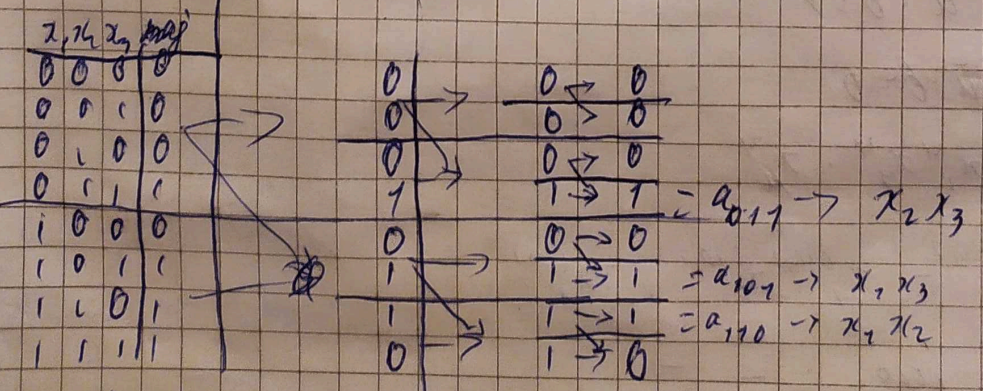
\includegraphics[width=0.5\linewidth]{images/image.png}
    \caption{Перетворення в АНФ}
    \label{fig:discrette_math:ANF-computation}
\end{figure}

\begin{equation*}
    maj(x_1, x_2, x_3) =  x_2 x_3 \oplus x_1 x_3 \oplus x_1 x_2.
\end{equation*}

\begin{example}
    $a_{101}$ - ? Вектор $101$ домінує над $000$, $100$, $001$ та $101$.
\end{example}

$\Rightarrow a_{101} = f(000) \oplus f(001) \oplus f(100) \oplus f(101) = 0 \oplus 0 \oplus 0 \oplus 1 = 1$

\subsection{Замкнені класи булевих функцій}

Замикання класу $\mathcal{F}$ -- множина всіх булевих функцій які реалізуються формулами над $\mathfrak{F}$, $[\mathcal{F}]$

Замкнений клас: $[\mathfrak{F}] = \mathcal{F}$

Повний клас: ${\mathcal{F}} = BF_n$

Базис -- повний клас і $\forall \mathcal{F}' \subset \mathcal{F}$, ($[\mathcal{F}'] \neq [\mathcal{F}]$)

$BF_n$ -- замкнений клас

$\mathcal{F}_A = \{\&, \oplus, 1\}$ -- базис

$\mathcal{F}_K = \{\&, \vee, \neg\}$ -- певний клас $x \vee y = \neg (x \& \overline{y})$.

$\{\&, \neg\}$ і $\{\vee, \neg\}$ -- базиси.

\subsection{Класи функцій}

Клас функцій що зберігають нуль
\begin{equation*}
    T_0 = \{f | f(0, 0, ..., 0) = 0\}.
\end{equation*}

Клас функцій які збурігають одиницю
\begin{equation*}
    T_1 = \{f | f(1, 1, ..., 1) = 1\}.
\end{equation*}

Клас самодвоїстих функцій
\begin{equation*}
    S = \{f | f = f^*\}.
\end{equation*}

Клас афінних (лінійних) функцій
\begin{equation*}
    A = \{f | f(x_1, x_2, ..., x_n) = a_0 \oplus a_1 x_1 \oplus ... \oplus a_n x_n\}, a \in \{0. 1\}.
\end{equation*}

Клас монотонних функцій
\begin{equation*}
    M = \{f | \forall x, y \in V_n x \prec y \Rightarrow f(x) \preceq f(y)\}.
\end{equation*}

\begin{lemma}
    Класи $T_0$, $T_1$, $S$, $A$, $M$ не вкладаються один у інший
\end{lemma}

\begin{example}
    \begin{tabular}{c|c|c|c|c|c}
        & $T_0$ & $T_1$ & $S$ & $A$ & $M$ \\\hline
        0 & + & - & - & + & + \\\hline
        1 & - & + & - & + & + \\\hline
        $\overline{x}$ & - & - & + & + & - \\\hline
        $maj$ & + & + & + & - & + \\
    \end{tabular}
\end{example}

\subsection{Критерій повноти системи булевих функцій}

\begin{claim}
    Класи $T_0$, $T_1$, $S$, $A$, $M$ є замкнені.
\end{claim}
\begin{proof}
    page 72 --------------------------
\end{proof}

-- замкнений

-- замкнений

-- замкнений

-- замкнений

-- замкнений


-- замкнений


Необхідна і достатня умова того, що система булевих функцій є повною

Якщо  то з  підстановкою  або  можна одержати константу

Приклад

Лемма 2 
Якщо  то  підстановкою  можна одержати 

Монотонність
Якщо  та  відрізняються лише у  бітах, то можна побудувати послідовність

та  , відрізняються в одному біті

Приклад

лемма3 
Якщо  тоді  підстановкою  або інвертуваннями її значення, можна отримати 
афінна  АНФ містить доданок із не менше ніж з двома змінними.

Нехай це змінна  та 

Нехай так, щоб

Якщо  то
Якщо  то

Приклади

Теорема Пост

-- повна

Необхідність

Якщо 
Якщо -- замкнений, то

Достатність
Побудуємо константи 0 та 1

Якщо  , то 
То

Якщо 
За леммою1 
змінимо на заперечення отриману константу

За лемою 2 з констант ми можемо одержати заперечення

За лемою 3 з констант, заперечення та  отримуємо 

Наслідок1 Класи  -- передповні класи
(що не є повні, але будуть кошдобавити одну функцію)

За теоремою Поста не вистачає  для повноти

Наслідок 2
Всі замкнені класи ж підмножинами хоча б одног з класів

Наслідок 3
З повного класу  можна обрати повний підклас у якому буде не тільки ніж у функції

Приклади

-- базис

-- базис

-- базиси

Теорма Пост
Існує 40 типів замкнених класів булевих функцій

Загальна кількість класів замкнених булевих функцій -- зліченна

Лемма

Теорема Уорд Ланель

Клейтман та Марковських


\section{Вступ до теорії графів}

% \subsection{Визначення}

% \subsection{Типи графів та їх узагальнення}

% \subsection{Способи подання графів}

% \subsection{Приклади графів}

% \subsection{Алгебраїчні операції над графами}

% \subsection{Алгоритмічні операції над графами}


% \section{Маршрути у графах}


% \section{Зв'язність графів}


% \section{Дерева та коди Прюфера}


% \section{Пошук мінімальних шляхів у зважених графах}


% \section{Способи представлення зваженого графу (22)}

% \section{Ізоморфність графів (23)}

% \section{Орієнтований граф}

% \section{Ойлерові Графи}

% \section{Гамільтонові Графи}

% \section{двочасткові графи}

 \section{Абстрактні автомати}

 \section{Формальні граматики}
 






